\documentclass[10pt]{article}
\usepackage{amsmath, amsthm, amssymb, mathtools}
\usepackage{hyperref}
\usepackage{aliascnt}
\usepackage{xcolor}

\title{Survey in Geometry}
\author{Dina Syverud-Lindland and Trym Erlend Bakkeland Lervik}
\date{}

% --- Theorem styles (italic body) ---
\theoremstyle{plain}
\newtheorem{theorem}{Theorem}[section]
\newtheorem{proposition}[theorem]{Proposition}
\newtheorem{lemma}[theorem]{Lemma}
\newtheorem{corollary}[theorem]{Corollary}

% --- Definition style (upright text) ---
\theoremstyle{definition}
\newtheorem{definition}[theorem]{Definition}
\newtheorem{example}[theorem]{Example}
\newtheorem{problem}{Problem}

% --- Remark style ---
\theoremstyle{remark}
\newtheorem{remark}[theorem]{Remark}

% --- Custom QED symbols ---
\renewcommand{\qedsymbol}{$\square$} % proofs end with □
% Custom end symbols for non-proof environments
% \renewcommand{\endmarker}{\hfill $\blacksquare$}

% Patch environments to end with ■
\usepackage{etoolbox}

\AtEndEnvironment{definition}{\hfill $\blacksquare$}
\AtEndEnvironment{example}{\hfill $\blacksquare$}
\AtEndEnvironment{problem}{\hfill $\blacksquare$}
\AtEndEnvironment{remark}{\hfill $\blacksquare$}

\usepackage{enumitem}
\setlist[enumerate]{label=(\roman*)}

\setlength{\parskip}{0pt}

\numberwithin{equation}{section}

\begin{document}

\setlist{nosep}

\maketitle
\noindent \textit{Transcription of lectures given by Prof. Ryosuke Takahashi at Tohoku University Spring 2026.}
\newpage
\tableofcontents
\newpage
\section{Review of differentiable manifolds}

\begin{definition}[n-dimensional differentiable manifold]
An \emph{n-dimensional differentiable manifold} is a topological space $M$ 
with an open cover $\{U_{\alpha}\}_{\alpha}$ and maps
\[\{\phi_{\alpha} : U_{\alpha} \to \phi_{\alpha}(U_{\alpha})\subset\mathbb{R}^n\}_{\alpha \in \Lambda}\]
satisfying
\begin{enumerate}
    \item $\phi_{\alpha}(U_{\alpha})\subset\mathbb{R}^n$ is open and $\phi_{\alpha}:U_{\alpha} \to \phi_{\alpha}(U_{\alpha})$ is a homeomorphism.
    \item If $U_{\alpha}\cap U_{\beta}\neq \emptyset$, then the transition map $\phi_{\beta} \circ \phi_{\alpha}^{-1}$ is a diffeomorphism (between open subsets of $\mathbb{R}^n$).
\end{enumerate}
$\{(U_{\alpha}, \phi_{\alpha}) : \alpha \in \Lambda\}$ is called a \emph{coordinate neighborhood system} or \emph{atlas}.
\end{definition}

Some terminology
\begin{itemize}
\item $n = \operatorname{dim}M$ \emph{dimension} of $M$.
\item $\phi_{\alpha}$ \emph{coordinate map} or \emph{chart}.
\item $\phi_{\alpha} = (x^1, \dots, x^n)$ \emph{local coordinates} $x^i : U_{\alpha} \to \mathbb{R}$.
\end{itemize}

\begin{definition}[Compatible charts]
Assume $M$ is an n-differentiable manifold with atlas $\{(U_{\alpha}, \phi_{\alpha}) : \alpha \in \Lambda\}$. A chart $(U, \phi)$ is \emph{compatible} with the atlas if
$\{U_{\alpha}, \phi_{\alpha})\}_{\alpha \in \Lambda} \cup (U,\phi)$ is again an atlas.
The set of all such charts is called the \emph{maximal coordinate neighborhood system} (or \textit{atlas}) of $M$.
\end{definition}

Henceforth, we assume the atlases of $M$ are always maximal.

\subsection{Differential of maps and tangent spaces}

\begin{definition}[$C^{\infty}$]
Assume $M,N$ are differentiable manifolds. A map continuous $f:M\to N$ is \emph{$C^{\infty}$} at $p \in M$
if there exists charts $(U, \phi)$ around $p$ and $(V, \psi)$ around $f(p)$ such that $\psi \circ f \circ \phi^{-1}: \phi(U) \to \psi(V)$ is $C^{\infty}$.
\end{definition}

\begin{remark}
\begin{itemize}
\item $M = I \subset \mathbb{R}, c:I\to N$ is a $C^{\infty}$ curve.
\item $N = \mathbb{R}, f:M\to \mathbb{R}$ is a $C^{\infty}$ function.
\item $C^{\infty}(M):= \{C^{\infty}\text{ function on } M\}$.
\end{itemize}
\end{remark}

\begin{definition}[Tangent vector and tangent space]
A map $v: C^{\infty}(M) \to \mathbb{R}$ is a \emph{tangent vector} at $p \in M$ if for all $a,b\in\mathbb{R}$ and all $f,g \in C^{\infty}(M)$, we have
\begin{enumerate}
\item $v(af + bg) = av(f) + bv(g)$ (linearity).
\item $v(fg) = f(p)v(g) + g(p)v(f)$ (Leibniz rule).
\end{enumerate}
The set $T_pM : = \{v : v \text{ is a tangent vector at } p\}$ is the \emph{tangent space} to $M$ at $p$.
\end{definition}

\begin{definition}[Velocity vector]
Let $c:I \to M$ be a $C^{\infty}$ curve with $c(0) = p \in M$. The \emph{velocity vector} of $c$ at $p$ is the map $c'(0) \in T_pM$ defined by
\[c'(0)(f) = \frac{d}{dt}\bigg|_{t=0} (f \circ c)(t), \quad f \in C^{\infty}(M).\]
\end{definition}

\begin{definition}[Coordinate vector fields]
Let $(U,\phi)$ be a chart around $p$ with $\phi(p)=0$, $\phi=(x^1,\dots,x^n)$.
Define curves
\[
c_i(t) := \phi^{-1}(0,\dots,t,\dots,0).
\]
Then
\[
\left.\frac{\partial}{\partial x^i}\right|_p := c_i'(0).
\]
\end{definition}

\begin{theorem}
For $p \in M$ an n-differentiable manifold, the tangent space $T_pM$ is an n-dimensional vector space with basis $\{\frac{\partial}{\partial x^1}\big|_p, \dots, \frac{\partial}{\partial x^n}\big|_p\}$.
I.e.
\[T_pM = \operatorname{span}\left\{\left.\frac{\partial}{\partial x^1}\right|_p, \dots, \left.\frac{\partial}{\partial x^n}\right|_p\right\}.\]
\end{theorem}

\begin{definition}[Differential]
Let $f:M\to N$ be a $C^{\infty}$ map between differentiable manifolds. The \emph{differential} of $f$ at $p \in M$ is the map
$df_p: T_pM \to T_{f(p)}N$ defined by
\[df_p(v)(g) := (f\circ c)'(0), \quad c \in C^{\infty}, \quad c(0) = p \text{ and } c'(0) = v. \]
\end{definition}

\begin{remark}
$c$ in the above definition is not unique, but $df_p(v)$ is well-defined.
\end{remark}

\begin{definition}[Diffeomorphism]
Let $M,N$ be differentiable manifolds. $f:M\to N$ is a \emph{diffeomorphism} if
\begin{itemize}
\item $f$ is a bijection.
\item $f$ and $f^{-1}$ are $C^{\infty}$.
\end{itemize}
In this case, $M$ and $N$ are \emph{diffeomorphic}.
\end{definition}

\subsection{Diffeomorphism groups and quotient manifolds}

Let $M$ be an n-differentiable manifold.

\begin{definition}[$C^{\infty}$ transformation group]
A set of diffeomorphisms $\Gamma = {\gamma_i}_{i\in I}$ on $M$ is a \emph{$C^{\infty}$ transformation group} if
\begin{itemize}
    \item For all $\gamma_i, \gamma_j \in \Gamma$, we have $\gamma_i \circ \gamma_j \in \Gamma$.
    \item For all $\gamma_i \in \Gamma$, we have $\gamma_i^{-1} \in \Gamma$.
    \item The identity map $\operatorname{Id}_M$ is in $\Gamma$.
\end{itemize}
\end{definition}

\begin{definition}[Proper discontinuous transformation group]
A $C^{\infty}$ transformation group $\Gamma$ on $M$ is \emph{properly discontinuous} if for each $p \in M$, there exists a chart $(U, \phi)$ around $p$ such that 
\[\gamma_i \in \Gamma \setminus \{\operatorname{Id}_M\} \implies \gamma_i(U) \cap U = \emptyset \text{ for all } i \in I.\]
\label{def:properly_disc_transf_group}
\end{definition}

Let $\Gamma$ be a properly discontinuous transformation group on $M$.
For each $p \in M$, let $(U_p, \phi_p)$ be a chart around $p$ as in definition \ref{def:properly_disc_transf_group}.

\begin{lemma}
For all $p\in M$ and all $\gamma_i, \gamma_j \in \Gamma$ ($\gamma_i \neq \gamma_j$), we have $\gamma_i(U_p) \cap \gamma_j(U_p) = \emptyset$ or $\gamma_i(U_p) = \gamma_j(U_p)$.
\end{lemma}

\begin{proof}
    $\gamma_i \neq \gamma_j \implies \gamma_i^{-1}\circ\gamma_j\neq\operatorname{Id}_M$. Then, by defintition \ref{def:properly_disc_transf_group},
    $U_p \cap \gamma_i^{-1}\circ\gamma_j(U_p) = \emptyset \implies \gamma_i(U_p) \cap \gamma_j(U_p) = \emptyset$.
\end{proof}

\begin{definition}[Orbit equivalence relation]
Let $\Gamma$ be a group acting on $M$. Define a relation on $M$ by
\[
p \sim q \iff \exists \gamma \in \Gamma \text{ such that } q = \gamma(p).
\]
\end{definition}

\begin{proposition}
The relation $\sim$ is an equivalence relation.
\end{proposition}

\begin{definition}[Orbit]
The equivalence class of $p$,
\[
[p] = \{ \gamma(p) \mid \gamma \in \Gamma \} \in M/\sim,
\]
is  the \emph{orbit} of $p$.
\end{definition}

\begin{definition}[Quotient manifold]
The quotient set $M/\Gamma := M/\sim$ is called the \emph{quotient manifold} of $M$ by $\Gamma$.
\begin{itemize}
    \item $M/\Gamma$ is equipped with the quotient topology via the projection map $\pi: M \to M/\Gamma$.
    \item $D \subset M$ is a \emph{fundamental domain} if $\pi|_D:D \to M/\Gamma$ is surjective.
\end{itemize}
\end{definition}

To show that $M/\Gamma$ is a differentiable manifold, we construct charts.
For $p \in M$, let $\hat{U}_p := \pi(U_p) \subset M/\Gamma$.

\begin{lemma}
If $q, r \in U_p$ satisfy $q \sim r$ then $q = r$. In particular, $\pi|_{U_p}: U_p \to \hat{U}_p$ is a
bijection.
\end{lemma}

\begin{proof}
$q \sim r \implies \exists \gamma_i \in \Gamma : r = \gamma_i(q) \in \gamma_i(U_p)$.
Thus $r \in \gamma_i(U_p)$ for some $\gamma_i \in \Gamma$.
Since $\Gamma$ is properly discontinuos, $\gamma_i = \operatorname{Id}_M$.
Hence, $r = \gamma_i(q) = q$. The second claim follows from $\pi(q) = \pi(r) \iff q \sim r$.
\end{proof}

\begin{problem}
Define $\hat{\phi}:\hat{U}_p \to \hat{\phi}_p(\hat{U}_p) = \phi_p(U_p) \subset \mathbb{R}^n$ by
\[\hat{\phi}_p := \phi_p \circ (\pi|_{U_p})^{-1}.\]
Show that $\hat{\phi}_p$ is a homeomorphism.
(Hint: In general, quotient maps are not necessarily open; use the proply discontinous property).
\end{problem}

\begin{theorem}
$\{(\hat{U}_p, \hat{\phi}_p) : p \in M\}$ is an atlas for $M/\Gamma$. Hence, $M/\Gamma$ is a differentiable manifold.
\end{theorem}

\subsection{Topology of differentiable manifolds}

Recall the convergence of a sequence $\{p_i\}_{i=1}^{\infty}$:
\[\lim_{i\to \infty} p_i = p \iff \forall \text{ open } O \ni p, \exists i_0 \in \mathbb{N} : i > i_0 \implies p_i \in O.\]

\begin{proposition}[Convergence in differentiable manifolds]
$\lim_{i\to\infty} p_i = p$ if and only if for every chart $(U, \phi)$ around $p$, we have $\lim_{i\to\infty} \phi(p_i) = \phi(p)$ (in $\mathbb{R}^n$).
That is, 
\[\lim_{i\to\infty} p_i = p \iff \forall (U, \phi) \exists i_0 \in \mathbb{N} : i > i_0 \implies \phi(p_i) \to \phi(p).\]
\end{proposition}

\begin{remark}
$M$ is Haussdorff and second countable and locally Euclidean. 
Thus, $f: M \to N$ is continuous at $p \in M$ if and only if $p_i \to p$ implies $f(p_i) \to f(p)$.
\end{remark}

\begin{lemma}
Let $(U,\phi)$ be a chart, $c:(a,b) \to M$ be a $C^{\infty}$ curve and $t_0 \in (a,b)$ that satisfy 
\begin{enumerate} 
    \item The map $\phi \circ c: (a,b) \to \mathbb{R}^n$ is $C^{\infty}$.
    \item $\exists \{t_i\}_{i=1}^{\infty} \subset (a,b) : t_i \to t_0$ and $t_i \geq t_0$ and $c(t_i) \notin U$.
\end{enumerate}
Then
\begin{enumerate}
    \item $c(t_0) \notin U$.
    \item $\forall \{s_i\}_{i=1}^{\infty} \subset (a,b) : s_i \to t_0$ and $s_i < t_0$, $(\phi \circ c)(s_i)$ does not converge in $\phi(U)$.
    \label{num}
\end{enumerate}
\end{lemma}

\begin{proof}
(1) Assume $c(t_0) \in U$. 
By continuity, $\exists \delta_0 > 0$ such that $c((t_0 - \delta_0, t_0 + \delta_0)) \subset U$.
For sufficiently large $i$, we have $t_i \in (t_0, t_0 + \delta_0) \implies c(t_i) \in U$, which contradicts \ref{num}.
(2) Assume $\exists \{s_i\} \to t_0$ ($s_i < t_0$) such that $\{\phi \circ c(s_i)\}$ converges in $\phi(U)$.
Then $(\phi \circ c)(s_i) \to x_0$ for some $x_0 \in \phi(U)$. By continuity of $\phi^{-1}$,
$c(s_i) = (\phi^{-1} \circ \phi)(c(s_i)) \to \phi^{-1}(x_0)$ as $i \to \infty$. By the continuity of $c$, we have $c(s_i) \to c(t_0)$ as $i \to \infty$. 
Since $M$ is Haussdorff, the limit is unique, so $\phi^{-1}(x_0) = c(t_0)$. Thus, $c(t_0) = \phi^{-1}(x_0) \in U$, which contradicts (1).
\end{proof}

\subsection{Tangent bundle}

Let $M$ be a differentiable manifold.

\begin{definition}[Tangent bundle]
The \emph{tangent bundle} of $M$ is the set
\[TM := \bigsqcup_{p \in M} T_pM = \{(p,v) : p \in M, v \in T_pM\}.\]
\end{definition}

We introduce a differentiable structure on $TM$ using the following framework:

\begin{problem}
Let $\{X_{\lambda}, \mathcal{O}_{\lambda}\}_{\lambda \in \Lambda}$ be a family of topological spaces satisfying the \emph{gluing axiom}:
\begin{align}
X_{\lambda} \cap X_{\mu} \neq \emptyset \implies
\begin{aligned}
&\text{the relative topologies from } X_{\lambda} \text{ and } X_{\mu} \text{ coincide on } X_{\lambda} \cap X_{\mu},\\
&\text{and } X_{\lambda} \cap X_{\mu} = \mathcal{O}_{\lambda} \cap \mathcal{O}_{\mu}.
\end{aligned}
\label{eq:gluing_axiom}
\end{align}
Set $X := \bigsqcup_{\lambda \in \Lambda} X_{\lambda}$.
\begin{enumerate}[label=(\arabic*)]
\item Show that $\mathcal{O} := \{U \subset X : X_{\lambda} \cap U \in U_{\lambda} \forall \lambda \in \Lambda\}$ is a topology
on $X$.
\item Show that the relative topology on $X_{\lambda}$ from $(X, \mathcal{O})$ coincides with $\mathcal{O}_{\lambda}$ for each $\lambda \in \Lambda$.
\label{prob:2.2}
\end{enumerate}
\label{prob:2}
\end{problem} 

\begin{remark}
The gluing axiom \ref{eq:gluing_axiom} is necessary for \ref{prob:2.2} and to ensure $X_{\lambda} \in \mathcal{O}$. Such a topology $\mathcal{O}$ is uniquely determined
by the base $\bigcup_{\lambda \in \Lambda} \mathcal{O}_{\lambda}$.
\end{remark}

Let $(U, \phi)$ be any chart on $M$ and set
\[TU := \bigsqcup_{p \in U} T_pM = \{(p,v) : p \in U, v \in T_pM\} \subset TM.\]
Define $\tilde{\phi}: TU \to \phi(U) \times \mathbb{R}^n \subset \mathbb{R}^{2n}$ as follows:
For $p \in U$, $v \in T_pM$, let $\phi(p) = (x_1, \ldots, x_n)$ and $v = \sum_{i=1}^n v_i\partial_i$, then
\[\tilde{\phi}(p,v) := (x_1, \ldots, x_n, v_1, \ldots, v_n).\]

\begin{theorem}
\begin{enumerate}[label=(\arabic*)]
\item The family of topological spaces $\{TU\}$ satisfies the gluing axiom \ref{eq:gluing_axiom}.
Thus, $TM = \bigsqcup_{(U,\phi)} TU$ is a topological space with the topology definited in problem \ref{prob:2}.
\item $TM$ is a $2n$-dimensional manifold with atlas $\{(TU, \tilde{\phi})\}$.
\item The projection $\pi:TM \to M$ defined by $\pi(p,v) := p$ for $v \in T_pM \quad (p \in M)$ is a $C^{\infty}$ map.
\end{enumerate}
\end{theorem}
\section{Tensors and Tensor Fields}

\subsection{Tensor Algebra}

We generalize bilinear forms to multilinear forms.

\begin{definition}[Multilinear map and multilinear function]
Let $V_1, \dots, V_k$ and $W$ be real vector spaces. A map
\[
f: V_1 \times \dots \times V_k \to W
\]
is \emph{multilinear} if it is linear in each component. For example,
\[
f(a v_1 + b w_1, v_2, \dots, v_k)
= a f(v_1, v_2, \dots, v_k) + b f(w_1, v_2, \dots, v_k)
\]
for all $a,b\in\mathbb{R}$ and $v_1,w_1\in V_1$. If $W=\mathbb{R}$, $f$ is called a \emph{multilinear function}.
\label{def:multilinear}
\end{definition}

\begin{definition}[$(s,t)$-type tensor]
Let $V$ be an $n$-dimensional real vector space and $V^*$ its dual.

For $s,t \in \mathbb{Z}_{\ge 0}$, a multilinear map
\[
T : (V^*)^s \times V^t \to \mathbb{R},
\]
is called a \emph{tensor of type} $(s,t)$. The set of all such tensors is denoted by $T_t^s(V)$; it is a real vector space under pointwise addition and scalar multiplication.
\end{definition}

\begin{remark}
Since the evaluation map $V \to V^{**}$
$v^{**}(f):= f(v)$ is a linear isomorphism,
it is sufficient to consider only $V^*$ and $V$ in definition \ref{def:multilinear} 
\end{remark}

\begin{problem}
For a multilinear map $T: (V^*)^s \times V^t \to \mathbb{R}$, define $\hat{T} \in T_t^{s+1}(V)$ by
\[
\hat{T}(\omega^1, \dots, \omega^{s+1}, v_1, \dots, v_t)
:= \omega^{s+1}\bigl(T(\omega^1, \dots, \omega^s, v_1, \dots, v_t)\bigr),
\]
where $\omega^1, \dots, \omega^{s+1} \in V^*$ and $v_1, \dots, v_t \in V$.
Show that the map $T \mapsto \hat{T}$ is a linear isomorphism.
\end{problem}

\begin{definition}[Tensor product]
For $T \in T_t^s(V)$ and $S \in T_{t'}^{s'}(V)$, define $T \otimes S \in T_{t+t'}^{s+s'}(V)$ by
\[
\begin{aligned}
(T \otimes S)&(\omega^1, \dots, \omega^{s+s'}, v_1, \dots, v_{t+t'})\\
&:=\; T(\omega^1, \dots, \omega^s, v_1, \dots, v_t) 
\times\; S(\omega^{s+1}, \dots, \omega^{s+s'}, v_{t+1}, \dots, v_{t+t'}),
\end{aligned}
\]
where $\omega^1, \dots, \omega^{s+s'} \in V^*$ and $v_1, \dots, v_{t+t'} \in V$.
\end{definition}

\begin{remark}
For any tensors $T, S, R$ and $a \in \mathbb{R}$, we have:
\begin{enumerate}
\item $\left(T \otimes S \right) \otimes R = T \otimes \left(S \otimes R\right)$.
\item $\left(aT\right) \otimes S = T \otimes \left(a S \right) = a \left(T \otimes S\right)$.
\end{enumerate}
These are denoted as $T \otimes S \otimes R$ and $a T \otimes S$, respectively.
Furthermore, $S$ and $R$ have the same type, the distributive laws hold :
\begin{enumerate}
    \item $T \otimes (S + R) = T \otimes S + T \otimes R$.
    \item $(S+R) \otimes T = S \otimes T + R \otimes T$.
\end{enumerate}
\end{remark}

\begin{remark}
In general, $S \otimes T \neq T \otimes S$.
\end{remark}

Let $\{e_i \}$ be a basis for $V$ and $\{e^i\}$ be its dual.
For $T \in T_t^s(V)$, the $n^{s+t}$ real numbers
\[
T^{i_1 \dots i_s}_{j_1 \dots j_t}
:= T(e^{i_1}, \dots, e^{i_s}, e_{j_1}, \dots, e_{j_t}),
\]
are called the \emph{coefficients} (or \emph{components}) of $T$.
For $T \in T_t^s(V)$ and $S \in T_{t'}^{s'}(V)$, the coefficients of $T \otimes S$ are given by
\[
 (T\otimes S)^{i_1 \dots i_{s+s'}}_{j_1 \dots j_{t+t'} }
 = T^{i_1 \dots i_s}_{j_1 \dots j_t} \; S^{i_{s+1} \dots i_{s+s'}}_{j_{t+1} \dots j_{t+t'}}.
\]

\begin{problem}
Show that the set of $n^{s+t}$ tensors
\[
e_{i_1} \otimes \dots \otimes e_{i_s} \otimes e^{j_1} \otimes \dots \otimes e^{j_t},
\]
where $i_1, \dots, i_s, j_1, \dots, j_t = 1, \dots, n$ 
forms a basis for $T_t^s(V)$; and that for any $T \in T_t^s(V)$,
\[
T = \sum_{i_1, \dots, i_s, j_1, \dots, j_t} T_{j_1 \dots j_t}^{i_1 \dots i_s} e_{i_1} \otimes \dots \otimes e_{i_s} \otimes e^{j_1} \otimes \dots \otimes e^{j_t}.
\]
In particular, show that $\dim T_t^s(V) = n^{s+t}$. We often write 
\[
T_t^s(V) = V \otimes \dots \otimes V \otimes V^* \otimes \dots \otimes V^*.
\]
\end{problem}

\subsection{Exterior Algebra}

\begin{definition}[p-form]
    Let V be a real vector space and $p \in \mathbb{N}$.
    An element of $T_p^0(V)$ is called a \emph{p-form}.
\end{definition}
\begin{remark}
A p-form $\omega$ is \emph{skew symmetric}. That is,
\[
\omega(v_{\sigma(1)}, \dots, v_{\sigma(p)}) = \text{sgn}(\sigma) \omega(v_1, \dots, v_p),
\]
for any $v_1, \dots, v_p \in V$ and $\sigma \in S_p$.
Furthermore, 
$\Lambda^p V^* := \{ \text{skew symmetric p-forms} \}$ is a vector space.
\end{remark}

\begin{definition}[Exterior product]
    For $\alpha \in \Lambda^p(V^*)$ and $\beta \in \Lambda^q(V^*)$, 
    the \emph{exterior product} $\alpha \wedge \beta$ is defined by 
    \[
    \alpha \wedge \beta := \frac{1}{p! q!} \sum_{\sigma \in S_{p+q}} \text{sgn}(\sigma) \alpha \otimes \beta \left(v_{\sigma(1)}, \dots, v_{\sigma(p+q)}\right).
    \]
\end{definition}

\begin{proposition}\label{prop:exterior_product}
    Let $\alpha, \alpha^1, \alpha^2 \in \Lambda^p(V^*)$ and $\beta, \beta^1, \beta^2 \in \Lambda^q(V^*)$.
    \begin{enumerate}
        \item $\left( a \alpha^1 + b \alpha^2 \right) \wedge \beta = a \alpha^1 \wedge \beta + b \alpha^2 \wedge \beta$.
        \item $\alpha \wedge \left( a \beta^1 + b \beta^2 \right) = a \alpha \wedge \beta^1 + b \alpha \wedge \beta^2$.
        \item $\left(\alpha \wedge \beta \right) \wedge \gamma = \alpha \wedge \left( \beta \wedge \gamma \right)$.
        \item $\beta \wedge \alpha = (-1)^{pq} \alpha \wedge \beta$.
    \end{enumerate}
\end{proposition}

\subsection{Tensor Fields and differential forms on manifolds}

Let M be an n-dimensional manifold an $\left( V, \phi \right)$ a chart with
$\phi = (x^1, \dots, x^n)$. At each $p \in U$, applying \autoref{prop:exterior_product} with $V = T_pM$, yields
\[
\frac{\partial}{\partial x^{i1}} \otimes \dots \otimes \frac{\partial}{\partial x^{is}} \otimes dx^{j1} \otimes \dots \otimes dx^{jt},
\]
which forms a basis for $T_t^s(T_pM)$. Any $T_p \in T_t^s (T_pM)$ can be written as,
\[
T_p = \sum_{i_1, \dots, i_s, j_1, \dots, j_t} T_{j_1 \dots j_t}^{i_1 \dots i_s} \frac{\partial}{\partial x^{i_1}} \otimes \dots \otimes \frac{\partial}{\partial x^{i_s}} \otimes dx^{j_1} \otimes \dots \otimes dx^{j_t}.
\]

\begin{definition}[$(s,t)$-type tensor field]
A map $T: M \owns p \to T_p \in T_t^s(T_pM)$ is a\emph{(s,t)-type tensor field}. $T$ is $C^{\infty}$ if all its coefficients 
$T_{j_1 \dots j_t}^{i_1 \dots i_s}$ are $C^{\infty}$ functions on any chart $(V, \phi)$.
\end{definition}

\begin{remark}
It suffices to check the $C^{\infty}$ property on a single atlas.
\end{remark}





\section{Riemannian metric}

Assume that $M$ is Hansforff differentiable manifold.
\begin{definition}[Riemannian metric and Riemannian manifold]
    A \emph{Riemannian metric} $g$ is a map
    \[
        M \owns p \to \langle \cdot, \cdot \rangle_p =: g_p ( \cdot, \cdot ) \text{that assigns a},
    \]
    (postive definite) inner product to each $T_pM$.
    The pair $\left(M, g\right)$ is called a \emph{Riemannian manifold}.
    In terms of tensor field, $g$ is a $(0,2)$-type tensor field (or a 2-form) on $M$.
\end{definition}

\begin{definition}[Length and angle]
For $v,w \in T_p M$, we have the following notions of length and angle:
\begin{itemize}
    \item \emph{Length} $\|v\| := \sqrt{\langle v, v \rangle}$.
    \item \emph{Angle} : $\theta \in [0,\pi]$ such that $cos \theta = \frac{\langle v, w \rangle}{\|v\| \|w\|}$.
\end{itemize}
\end{definition}

\begin{example}
Let $(v, \phi)$ be a chart with
\[
\phi = (x^1, \dots, x^n).
\]
Define $g_{ij} : U \to \mathbb{R}$ by
\[
g_{ij}(p) :=  \left\langle \left(\frac{\partial}{\partial x^i}\right)_p, \left(\frac{\partial}{\partial x^j}\right)_p \right\rangle.
\]
On $U$, $g$ is expressed as 
\[
g = \sum_{i,j=1} g_{ij} dx^i \otimes dx^j.
\]
The matrix $(g_{ij})$ is a postive definite symmetric matrix.
\[
ds^2 = \sum_{i,j =1}^n \delta_{ij} dx^i \otimes dx^j = \sum_{i=1}^n (dx^i)^2.
\]
\end{example}

\begin{problem}
Consider two charts $(U, \phi)$ and $(V, \psi)$ with $U \cap V \neq \emptyset$. 
\[
\phi = (x^1, \dots, x^n), \psi = (y^1, \dots, y^n),
\]
and let $g_{ij}$, $\hat{g}_{kl}$ be the components of g with respect to these charts.
Show that on $U \cap V$ satisfies the following transformation law:
\[
\hat{g}_{kl} = \sum_{i,j=1}^n g_{ij} \frac{\partial x^i}{\partial y^k} \frac{\partial x^j}{\partial y^l}.
\]
\end{problem}

\begin{definition}[$C^{\infty}$ Riemannian manifold]
$(M,g)$ is a \emph{$C^{\infty}$ Riemannian manifold} if $g$ is a $C^{\infty}$ tensor field.
\end{definition}
\begin{proposition}
The following are equivalent:
\begin{itemize}
    \item (M,g) is a $C^{\infty}$ Riemannian manifold.
    \item Copmonents $g_{ij}$ are $C^{\infty}$ functions for any chart $(U, \phi)$.
    \item $p \to \langle X_p, Y_p \rangle$ is $C^{\infty}$ for any $C^{\infty}$ vector fields $X,Y$.
\end{itemize}    
\end{proposition}
Henceforth, assume that all Riemanninan metrics are $C^{\infty}$.
\begin{remark}
$g,h$ : Riemannian metric, $f \in c^{\infty} ( M, \mathbb{R}_{>0})$
$\implies$ $fg$ and $g+h$ are also Riemannian metrics.
\end{remark}

\begin{proposition}
    Every paracompact manifold admits a Riemannian metric.
\end{proposition}

\begin{proof}
    Let $\{(U_k, \phi_k)\}_{k=1}^{K_0}$ be a finite atlas and let $\{x_k\}^{K_0}_{k=1}$
    be a partition of unity subordinate to ${U_k}$. On $U_k$, define $g_k$
    \[
    g_k(u,w) := \langle(d \phi_k)_p(v), (d \phi_k)_p (w) \rangle_{\mathbb{R}^n}, v,w \in T_pM.
    \]
    Then the global metric is given by:
    \[
    g := \sum_{k=1}^{K_0} x_k g_k
    \]
\end{proof}

\subsection{Isometries}

\begin{definition}[Isometry]
Let $(M,g)$ and $(N,h)$ be Riemannian manifolds and let $f : M \to N$ be a smooth map.
\begin{itemize}
\item The map $f$ is called \emph{locally isometric} if
\[
\langle (df)_p(v), (df)_p(w) \rangle_{f(p)} = \langle v, w \rangle_p
\quad \text{for all } p \in M, \; v,w \in T_pM.
\]
\item The map $f$ is called an \emph{isometry} if it is a diffeomorphism and locally isometric.
\item The manifolds $M$ and $N$ are called \emph{isometric} if there exists an isometry $f : M \to N$.
\end{itemize}
\end{definition}

\begin{proposition}
\begin{enumerate}[label=(\arabic*)]
\item $f: L \to M, h : M \to N$ are (local) isometric maps $\implies h \circ f$ is a (local) isometric map.
\item $f$ is isometry $\implies f^{-1}$ is isometry.
\end{enumerate}
Thus, the relation "Isometric" is an equivalence relation.
\end{proposition}

\subsection{Riemannian submanifold}

\begin{definition}[Riemannian submanifold]
Assume $M$ is a Riemannian manifold and $N \subset M$ is a submanifold.
$N$ is a \emph{Riemannian submanifold} if the metric is defined by $\langle v, w \rangle_N := \langle v, w \rangle_M$ for all $v, w \in T_pN$.
\end{definition}

The inclusion $C : N \to M$ is always an isometric map.

\subsubsection{Remember 3.10 Nash Embedding Theorem}
Every Riemannian manifold is isometric to a riemannian submanifold of some Euclidian space $\mathbb{R}^n$. $\Leftrightarrow$
\emph{Whitney Embedding Theorem}
\section{Length of curves and Riemann distance}

Let $M$ be a Riemannian manifold, $I \subset \mathbb{R}$ be an interval, and $c:I\to M$ a $C^{\infty}$ curve.
\begin{definition}[Length of a curve]\label{def:length_of_curve}
For $a,b\in I$ such that $a<$, the \emph{length} $L(c|_{[a,b]})$ of $c$ on $[a,b]$ is defined by
\[
L(c|_{[a,b]}) := \int^b_a ||c'(t)|| dt.
\]
\textcolor{red}{Here, I believe $||\dots|| = \sqrt{\langle \dots, \dots \rangle}$.}
\end{definition}

\begin{definition}[Regular curve]
A $C^{\infty}$ curve $C:I\to M$ is \emph{regular} if
\[
c'(t) \neq 0, \quad \forall t \in I.
\]
\end{definition}

\begin{theorem}[Inverse function theorem for regular curves] \label{thm:inverse_function_theorem}
Assume that the parameter $t$ is a $C^{\infty}$ function of $u$ on $J \subset \mathbb{R}$, i.e. $t = t(u)$ satisfying:
\begin{enumerate}
\item $t: J \to I$ is surjective.
\item $\frac{dt}{du}(u) \neq 0 \forall u \in J$.
\end{enumerate}
Then there exists a $C^{\infty}$ inverse $t^{-1}: I \to J$. This is called a \emph{transformation of parameter} $t$ to $u$.
\end{theorem}

Let $\tilde{c} := c(t(u))$ be a reparametrization of $c$ by $t$. Fix a chart $(U, \phi), \phi = (x^1, \dots, x^n)$ and subinterval $I'\subset I$ such that $c(I')\subset U$.
For $t \in I'$ and $u\in t^{-1}(I')$, let
\[
\phi(c(t)) = (c^1(t), \dots, c^n(t)), \quad \phi(\tilde{c}(u)) = (\tilde{c}^1(u), \dots, \tilde{c}^n(u)).
\]
Since $\tilde{c}^i(u) = c^i(t(u))$, we have
\[
\begin{aligned}
\tilde{c}'(u) &= \sum_{i=1}^n \frac{d\tilde{c}^i}{du}\left(\frac{\partial}{\partial x^i}\right)_{\tilde{c}(u)} \\
&= \sum_{i=1}^n \frac{dt}{du} \frac{dc^i}{dt}(t(u))\left(\frac{\partial}{\partial x^i}\right)_{\tilde{c}(u)}\\
&= \frac{dt}{du} c'(t(u)).
\end{aligned}
\]
Since $(U,\phi)$ was arbitrary, for all $u \in J$,
\[
\tilde{c}'(u) = c'(t(u))\frac{dt}{du}.
\]
\begin{proposition}
Let $c:I\to M$ be a regular curve and $t = t(u)$ ($u \in J$) be a transformation. Then
\begin{enumerate}[label=(\arabic*)]
\item If $\frac{dt}{du}(u) > 0 $ ($\forall u \in J$), then $L(\tilde{c}|_{[a,b]}) = L(c|_{[t(a),t(b)]}) \forall a,b \in J (a < b)$.
\item If $\frac{dt}{du}(u) < 0 $ ($\forall u \in J$), then $L(\tilde{c}|_{[a,b]}) = L(c|_{[t(b),t(a)]}) \forall a,b \in J (a < b)$.
\end{enumerate}
\end{proposition}
\begin{proof}
\begin{enumerate}[label=(\arabic*)]
\item By \autoref{def:length_of_curve} (length of a curve),
\[
\begin{aligned}
L(\tilde{c}|_{[a,b]}) &= \int^b_a ||\tilde{c}'(u)|| du \\
&= \int^b_a ||c'(t(u))|| \left|\frac{dt}{du}\right| du \\
&= \int^{t(b)}_{t(a)} ||c'(t)|| dt \\
&= L(c|_{[t(a),t(b)]}).
\end{aligned}
\]
\item Again, by \autoref{def:length_of_curve},
\[
\begin{aligned}
L(\tilde{c}|_{[a,b]}) &= \int^b_a ||\tilde{c}'(u)|| du \\
&= \int^b_a ||c'(t(u))|| \left|\frac{dt}{du}\right| du \\
&= \int^{t(a)}_{t(b)} ||c'(t)|| dt \\
&= L(c|_{[t(b),t(a)]}).
\end{aligned}
\]
\end{enumerate}
\end{proof}

\begin{definition}[Arclength parameter]
A regular curve $c:I\to M$ is said to have an \emph{arclength parameter} $s$ if $||c'(s)|| = 1$ for all $s \in I$.
\end{definition}
If $c:I\to M$ has an arclength parameter, then
\[
L(c|_{[a,b]}) = \int^b_a ||c'(s)|| ds = \int^b_a 1 ds = b-a, \quad \forall a,b \in I (a < b).
\]
Meaning the "elapsed time" $b-a$ equals the distance traveled along $L(c|_{[a,b]})$.
For any regular curve $c:I\to M$ and $t_0 \in I$, let
\[
s(t) := \int^t_{t_0} ||c'(t)|| dt.
\]
Since $\frac{ds}{dt} = ||c'(t)|| > 0 \implies$ there exists a global inverse $t=t(s)$ by \autoref{thm:inverse_function_theorem} (inverse function theorem).

\begin{lemma}
$\tilde{c}(s) = c(t(s))$ has an arclength parameter $s$.
\end{lemma}
\begin{proof}
By $\tilde{c}'(s) = c'(t(s)) \frac{dt}{ds}$, we have
\[
\begin{aligned}
||\tilde{c}'(s)|| &= ||c'(t(s))|| \left|\frac{dt}{ds}\right|,\\
\left|\frac{dt}{ds}\right| &= \frac{1}{\frac{ds}{dt}} = \frac{1}{||c'(t)||}.
\end{aligned}
\]
Meaning we have $||\tilde{c}'(s)|| = 1$ for all $s \in I$.
\end{proof}

\begin{definition}[Piecewise smooth curve]
A continuous curve $c:[a,b]\to M$ is a \emph{piecewise smooth regular curve} if there exists a finite sequence $a = t_0 < t_1 < \dots < t_k = b$ such that
\[
c|_{[t_,t_{i+1}]}:[t_i,t_{i+1}] \to M
\]
is regular for all $i = 0, \dots, k-1$.

Furthermore, the length $L(c)$ is defined by
\[
L(c) := \sum^{k-1}_{i=0} L(c|_{[t_i,t_{i+1}]}) = \sum^{k-1}_{i=0} \int^{t_{i+1}}_{t_i} ||c'(t)|| dt.
\]
\end{definition}

Assume $M$ is connected, i.e. any two points are joinable by a regular curve.
\begin{definition}[Riemannian distance]
The \emph{Riemannian distance} $d(p,q)$ between two points $p, q \in M$ is defined as
\[
d(p,q) := \inf \{ L(c) : c \text{ is a piecewise smooth regular curve from } p \text{ to } q \}.
\]
$d:M\times M \to \mathbb{R}$ is called the \emph{Riemannian distance function}.
If there exists some function $c$ attaining the "inf", then $c$ is called a \emph{minimal curve}.
\end{definition}

\begin{theorem}
The function $d:M\times M \to \mathbb{R}$ is satisfies the axioms of distance. That is, for all $p,q,r \in M$,
\begin{enumerate}[label=(\arabic*)]
\item $d(p,q) = 0$ if and only if $p=q$,
\item $d(p,q) = d(q,p)$,
\item $d(p,r) \leq d(p,q) + d(q,r)$.
\end{enumerate}
\label{thm:distance_axioms}
\end{theorem}

\begin{lemma}
$\left(U, \phi \right)$ : a chart, $D \subset \phi(U)$ a cpt set.
$c : [a,b] \rightarrow \phi^{-1} (D)$ : a piecewise smooth regular curve, Then $\exists C = C\left( (U, \phi), g_{ij}, D \right) >0$ s.t 
for $\bar{c} := \phi \circ c :[a,b] \rightarrow \mathbb{R}^n$
\[
\begin{aligned}
    C^{-1} L(\bar{c}) &\leq L(c) \leq C L(\bar{c}), \text{ where}\\
    L(\bar{c}) &= \int_a^b \|\bar{c}'(t)\|_{\mathbb{R}^n} dt \text{ is the Euclidean length.}
\end{aligned}
\]
\label{lemma:length_of_curve_in_chart}
\end{lemma}

\begin{proof}
    Define a continous function $f: \phi(u) \times \mathbb{R}^n \rightarrow \mathbb{R}$ by
    \[
    \begin{aligned}
        f(x,v) &:= \sum_{i,j = 1}^n v^i v^j g_{ij} (\phi^{-1}(x))
    \end{aligned}
    \]
    Since $D\times \mathbb{S}^{n-1} \subset \mathbb{R}~{2n}$ is cpt, $f|_{D \times \mathbb{S}^{n-1}}$ has max/min. Since $f>0$, the min is positive.
    \[
    \begin{aligned}
        \implies \exists C>0 \text{ s.t } c^{-2} \leq f \leq C^2 \text{ on } D \times \mathbb{S}^{n-1}
    \end{aligned}
    \]
    Thus, $\forall x \in D$ and $\forall v \in \mathbb{R}^n \setminus \{0\}:$
    \[
    \begin{aligned}
        C^{-2} \leq f\left(x, \frac{v}{\|v\|_{\mathbb{R}^n}} \right) \leq C^2
    \end{aligned}
    \]
    Multiplying $\|v\|^2_{\mathbb{R}^n}$
    \[
    \begin{aligned}
        C^{-2} \|v\|_{\mathbb{R}^n}^2 \leq \sum^n_{i,j=1} v^i v^j g_{ij}(\phi^{-1}(x)) \leq C^2 \|v\|_{\mathbb{R}^n}^2
    \end{aligned}
    \]
    Let $\bar{c} = \left(c^1(t), \dots, c^n(t)\right) \implies c'(t) = \sum^n_{i=1} \frac{dc^i}{dt} \partial_i$.
    \[
    \begin{aligned}
        \bar{c}'(t) &= \left(\frac{dc^1}{dt}, \dots, \frac{dc^n}{dt} \right). \text{ Set } v := \bar{c}'(t) \\
        &C^{-2} \| \bar{c}'(t)\|_{\mathbb{R}^n}^2 \leq \|c'(t)\|^2 \leq C^2 \|\bar{c}'(t)\|_{\mathbb{R}^n}^2
    \end{aligned}
    \]
    Taking square roots and integrating with respect to $t$ yields the result.
\end{proof}

\begin{lemma}
    Let $(U, \phi)$ be a chart of M.
    Choose $x_0 \in \phi(U)$ and $r>0$ s.t $D := \bar{B}(x_0, 3r) \subset \phi(U)$.
    Let $C>0$ be the constant from \autoref{lemma:length_of_curve_in_chart}. Then:
    \begin{enumerate}
        \item $\forall p,q \in \phi^{-1}({B}(x_0, r))$: \\
        $C^{-1} \| \phi(p) - \phi(q) \|_{\mathbb{R}^n} \leq d(p,q) \leq C \|\phi(p) - \phi(q)\|_{\mathbb{R}^n}$.
        \item $\forall p \in \phi^{-1}({B}(x_0, r)), \forall q \in M \setminus \phi^{-1}(D) : d(p,q) \leq 2C^{-1}r$
    \end{enumerate}
    \label{lemma:distance_in_chart}
\end{lemma}

\begin{proof}
    (1) $p,q \in \phi^{-1}({B}(x_0, r))$. $\bar{\gamma}$ : the line segment in $\mathbb{R}^n$ connecting $\phi(p)$ and $\phi(q)$. 
    Since $B(x_0, r)$ is convex, $\bar{gamma} \subset B(x_0, r)$. Set $\gamma := \phi^{-1} \circ \bar{\gamma}$.
    By \autoref{lemma:length_of_curve_in_chart},
    \[
    \begin{aligned}
        \|\phi(p) - \phi(q) \|_{\mathbb{R}^n} \leq L(\bar{\gamma}) \leq C^{-1} L(\gamma) \geq C^{-1} d(p,q).
    \end{aligned}
    \]
    Next, take any piecewise smooth refular curve $C: [0,l] \to M$ from $p$ to $q$. 
    If $c([0,l]) \subset \phi^{-1}(D)$, let $\bar{c} := \phi \circ c$. By \autoref{lemma:length_of_curve_in_chart},
    \[
    \begin{aligned}
        L(c) \geq C^{-1} L(\bar{c}) \geq C^{-1} \|\phi(p) - \phi(q)\|_{\mathbb{R}^n}.
    \end{aligned}
    \]
    If $c([0,l]) \not\subset \phi^{-1}(D)$, let
    \[
    \begin{aligned}
        t_1 := sup \{t\in [0,l] | c([0,t]) \subset \phi^{-1}(D)\}
    \end{aligned}
    \]
    and $c_1 := c|_{[0,t_1]}$. By \autoref{lemma:disjoint_or_equal}, $c_1(t_1) \in \phi^{-1}(\partial D)$
    Let $\bar{c}_1 := \phi \circ c_1$. By \autoref{lemma:length_of_curve_in_chart},
    \[
    \begin{aligned}
        L(c) \geq L(c_1) \geq C^{-1} L(\bar{c}_1).
    \end{aligned}
    \]
    Since $\phi(p), \phi(q) \in B(x_0, r )$ and $\bar{c_1}(t_1) \in \partial B(x_0, 3r)$
    \[
    \begin{aligned}
        &L(\bar{c_1}) \geq 2r > \|\phi(p)-\phi(q)\|_{\mathbb{R}^n} \\
       \implies &L(c) > C^{-1} \|\phi(p) - \phi(q)\|_{\mathbb{R}^n} \text{ in both cases}
    \end{aligned}\]
    Taking inf over c (using the fact that C in \autoref{lemma:length_of_curve_in_chart} is independent of c)
    \[
    \begin{aligned}
        d(p,q) \geq C^{-1} \|\phi(p) - \phi(q) \|_{\mathbb{R}^n}
    \end{aligned}
    \]
    (2) Prf is similar to (1) above (omitted).
\end{proof}

\begin{proof}[Proof of \autoref{thm:distance_axioms}]
    (1) $p=q \implies$ taking $c(t) = p$ gives $L(c) = 0 $ thus $d(p,q) =0$.
    conversely, assume $d(p,q) = 0$.
    Fix a xhart $(U, \phi)$ around $p$ and let $x_0 := \phi(p)$. 
    Choose $r>0$ s.t $D_r := \bar{B}(x_0, 3r) \subset \phi(U)$. By \autoref{lemma:distance_in_chart}, 
    \[
    \begin{aligned}
        \exists C_r > 0 \text{ s.t if } q \in M \setminus \phi^{-1} (D_r), \text{ then } d(p,q) \geq 2C_r^{-1} r
    \end{aligned}
    \]
    Contradicting $d(p,q) = 0$. Thus $q \in \phi^{-1}(D_r)$.
    Since $r>0$ is arbitrary, $p=q$

    (2) Let $c$ be a piecewise smooth regular curve from $p$ to $q$. Reversing, the parameter yiels a curve from $q$ to $p$ with the same length. $\implies d(p,q) = d(q,p)$

    (3) Let $c_{pq}$ be a curve from $p$ to $q$, and $c_qr$ from $q$ to $r$. Concatenating them yields a piecewise smooth regular curve from $p$ to $r$.
    $d(p,r) \leq L(c_{pqr}) = L(c_{pq}) + L(c_{qr})$ Taking inf over $c_{pq}$ and $c_{qr} \implies$ triangle inequality. 
\end{proof}

\begin{remark}
    Hausdorff property is essential for $d(p,q) = 0$. In non-Hausdorf manifolds, $d(p,q)=0$ does not necessarily imply $p=q$
\end{remark}

\begin{problem}
    Define $L, R_+, R_- \subset \mathbb{R}^2$ as:
    \[
    \begin{aligned}
        &L:= \{(x, 0) \in \mathbb{R}^2 | x<0\}\\
        &R_+ := \{(x, 1) \in \mathbb{R}^2 | x \geq 0\}, R_- := \{(x, -1) \in \mathbb{R}^2 | x \geq 0\}
    \end{aligned}
    \]
    $M:=L \cup R_+ \cup R_-$, $U:= L \cup R_+, V:= L \cup R_-$
    Let $\pi_1 : \mathbb{R}^2 \to \mathbb{R}$ be the projectioon to the 1st component
    and $\phi := \pi_1 |_U : U \to \mathbb{R}, \psi := \pi_1 |_V : V \to \mathbb{R}$
    $W \subset M$ is open : $\equiv \phi(W \cap U), \psi(W \cap  V)\subset \mathbb{R}$ are open.
    This makes $M$ a topological space s.t. $\phi, \psi$ are homeomorphisms,
    \[
    \begin{aligned}
        \phi(U \cap V) = \psi(U\cap V) = (-\infty, 0), \text{ and } \psi \circ \phi^{-1} = Id_{(-\infty, 0)}
    \end{aligned}
    \]
    \begin{enumerate}
        \item Show M is not Hausdorff
        \item Show $d \left((0,1), (0,-1)\right) = 0$ for any riemann metric on $M$
    \end{enumerate}
\end{problem}

\begin{definition}
    For $p\in M$, $r>0$
    \[
    \begin{aligned}
        B(p,r) := \{q \in M | d(p,q) < r\}
    \end{aligned}
    \]
    is called a geodesic ball of radius $r$ centered at $p$
\end{definition}

\begin{proposition}
    For a subset $O \subset M$ the following are equivalent:
    \begin{enumerate}
        \item $O$ is open in $M$
        \item $\forall p \in O, \exists \delta > 0 \text{ s.t. } B(p, \delta) \subset O$
    \end{enumerate}
    \label{prop:open_in_manifold}
\end{proposition}

\begin{proof}
    Take a chart $(U, \phi)$ around $p$ and let $x_0 := \phi(p)$. Since $\phi(O \cap U) \subset \mathbb{R}^n$ is open,
    $\exists \gamma > 0$ s.t. $D_i = \bar{B}(x_0, 3r) \subset \phi(O \cap U)$. For the constant $C>0$ from \autoref{lemma:distance_in_chart}, choose $\delta >0$ s.t.
    $0 < \delta < 2 C^{-1}r$. Then $\forall q \in M \setminus \phi^{-1}(D),$
    $d(p,q) \geq 2C^{-1}r > \delta$. Thus $q \in B(p, \delta) \implies q \in \phi^{-1}(D)$,
    we have $B(p,\delta) \subset O$.
    $(2) \implies (1)$ : Let ${(U_{\alpha}, \phi_{\alpha})}_{\alpha \in \Lambda}$ be an atlas of $M$. Then $O = \bigcup_{\alpha \in \Lambda} (O \cap U_{\alpha})$.
    Since each $\phi_{\alpha} : U_{\alpha} \to \phi_{\alpha} (U_{\alpha})$ is a homeo,
    $O \cap U_{\alpha}$ is open in $U_{\alpha} \equiv \phi_{\alpha} (O \cap U_{\alpha})$ is open in $\phi_{\alpha}(U_{\alpha})$.
    Thus it suffices to show: $\phi (O \cap U) \subset \mathbb{R}^n $ is open for any chart $(U, \phi)$

    $x \in \phi(O \cap U)$, set $p := \phi^{-1}(x) \in O \cap U$. By assumption, $\exists r_1 >0 \text{ s.t. } B(p, r_1) \subset O$.
    Since $\phi (U) \subset \mathbb{R}^n$ is open, $\exists r_2>0 \text{ s.t. } \bar{B}(x, 3 r_2) \subset \phi(U)$.
    For $(U, \phi)$ and $D := \bar{B}(x, 3 r_2)$ let $C>0$ be the constant from \autoref{lemma:length_of_curve_in_chart}. Set $r:= min{C^{-1}r_1, r_2}$.
    Then $B(p, C r) \subset B(p, r_1) \subset O$. For any $y \in B(x, r)$ set $q := \phi^{-1}(y) \in \phi^{-1}(B(x. r_2)) \subset U$. By \autoref{lemma:length_of_curve_in_chart}:
    \[
    \begin{aligned}
        d(p,q) \leq C \| x-y \|_{\mathbb{R}^n} < C r,
    \end{aligned}
    \]
    Thus $q \in B(p, Cr) \subset O$, which implies $q \in O \cap U$ and $y \in \phi(O \cap U)$. Therefore $B(x,r) \subset \phi(O \cap U)$ and $\phi(O \cap U)$ is open in $\mathbb{R}^n$
\end{proof}

\begin{problem}
    Using \autoref{prop:open_in_manifold}, show that for any $p \in M$ and $r>0$, the geodesic ball $B(p,r)$ is an open set in $M$.
    The following properties hold for distance functions on general metric spaces, thus proofs are omitted. $d: M \times M \to \mathbb{R}$.
    \begin{proposition}
        $\forall p_0 \in M$, $f(p) := d(p, p_0)$ is continous
    \end{proposition}
    \begin{proposition}
        For a sequence ${p_i}_{i=1}^{\infty} \subset M$ and $p\in M$, the following are equivalent:
        \begin{enumerate}
            \item $p_i \to p$ as $i \to \infty$
            \item $d(p_i, p) \to 0$ as $i \to \infty$
        \end{enumerate}
        Basic topological properties of geodesic balls (proofs omitted:)
    \end{proposition}
    \begin{proposition}
        $\forall p \in M$ and $r>0$
        \begin{enumerate}
            \item $\partial B(p,r) = {q \in M | d(p,q)=r}$
            \item $\bar{B}(p,r) := \bar(B(p,r)) = {q \in M | d(p,r) \leq r}$
        \end{enumerate}
    \end{proposition}
\end{problem}
\section{Levi-Civita connection}

Assume $M$ is a Riemannian manifold.

\begin{definition}[Levi-Civita connection]\label{def:5.1}
\[
\nabla : \underset{\in (X,Y)}{\mathcal{\mathfrak{X}(M)}\times\mathfrak{X}(M)} \to \underset{\in \nabla \times Y}{\mathfrak(M)}
\]
is called the \emph{covariant derivative} or \emph{Levi-Civita connection} if
$\forall X, Y, Z \in \mathfrak{X}(M)$ and $\forall f \in C^{\infty}(M)$:
\begin{enumerate}[label=(\arabic*), ref=Definition \thedefinition~(\arabic*)]
    \item \label{def:5.1.1} $\nabla_{X+Y}Z = \nabla_X Z + \nabla_Y Z$
    \item \label{def:5.1.2} $\nabla_{fX}Y = f\nabla_X Y$
    \item \label{def:5.1.3} $\nabla_X(Y+Z) = \nabla_X Y + \nabla_X Z$
    \item \label{def:5.1.4} $\nabla_X(fY) = X(f)Y + f\nabla_X Y$
    \item \label{def:5.1.5} $\nabla_X Y - \nabla_Y X = [X,Y]$ (torsion-free)
    \item \label{def:5.1.6} $X\langle Y, Z \rangle = \langle \nabla_X Y, Z \rangle + \langle Y, \nabla_X Z \rangle$ (metric compatibility)
\end{enumerate}
\end{definition}

\begin{theorem}[Fundamental theorem of Riemannian geometry]
There exists a unique ($\exists !$) Levici-Civita connection $\nabla$ on a Riemannian manifold $M$.
\end{theorem}

\begin{proof}\label{proof:fundamental_theorem_of_riemannian_geometry}
We start by showing uniqueness. By \autoref{def:5.1.6}:
\[
\begin{aligned}
    X\langle Y, Z \rangle &= \langle \nabla_X Y, Z \rangle + \langle Y, \nabla_X Z \rangle\\
    Y \langle Z, X \rangle &= \langle \nabla_Y Z, X \rangle + \langle Z, \nabla_Y X \rangle\\
    - Z \langle X, Y \rangle &= - \langle \nabla_Z X, Y \rangle - \langle X, \nabla_Z Y \rangle
\end{aligned}
\]
Summing over these and applying \autoref{def:5.1.5}:
\begin{align}\label{eq:levi-civita_uniqueness}
\langle \nabla_XY, Z\rangle &= \frac12 \{X\langle Y, Z \rangle + Y \langle Z, X \rangle - Z \langle X, Y \rangle + \langle [X,Y], Z \rangle \notag \\
& - \langle [Y,Z], X \rangle + \langle [Z,X], Y \rangle\}
\end{align}
This shows uniqueness.

We now show existence. Let the right-hand side of \eqref{eq:levi-civita_uniqueness} be $F_{X,Y}(Z)$.
Then $\forall f_1, f_2 \in C^{\infty}(M)$ and $\forall Z_1, Z_2 \in \mathfrak{X}(M)$:
\[
F_{X, Y}(f_1 Z_1 + f_2Z_2) = f_1F_{X,Y}(Z_1) + f_2F_{X,Y}(Z_2),
\]
is easily verified. For a chart $(U, \phi)$, we can define
\[
\nabla_X^{(U,\phi)}Y := \sum_{i, j = 1}^{n}F_{X,Y}(\partial_i)g^{ij}\partial_j,
\]
where $(g^{ij})=(g_{ij})^{-1}$. For $Z = \sum_{k=1}^n Z^k\partial_k$, using that $\sum_{j=1}^n g^{ij}g_{jk}=\delta^i_k$, we have
\[
\begin{aligned}
\langle \nabla_X^{(U,\phi)}Y, Z \rangle &= \sum_{i,j,k = 1}^n F_{X,Y}(\partial_i)g^{ij}Z^k g_{jk} \\
&= \sum_{i=1}^n F_{X,Y}(\partial_i)Z^i = F_{X,Y}(Z).
\end{aligned}
\]
Note that this is independent of the choice of chart $(U,\phi)$! This implies that for any other chart $(V, \psi)$ such that $U \cap V \neq \emptyset$, $\nabla_X^{U,\phi} = \nabla_X^{(V,\psi)}Y$.
Thus $\nabla_X Y := \nabla_X^{(U, \phi)}Y$ yields a globally defined vector field. Direct calculation verifies all axioms \autoref{def:5.1.1}--\autoref{def:5.1.6} of \autoref{def:5.1}.
\end{proof}

\begin{problem}
Verify axioms \autoref{def:5.1.1}--\autoref{def:5.1.6} of \autoref{def:5.1} for the Levi-Civita connection $\nabla$ constructed in \autoref{proof:fundamental_theorem_of_riemannian_geometry}.
\end{problem}

\begin{definition}[Christoffel symbols]\label{def:christoffel_symbols}
For a chart $(U,\phi)$, we define functions $\Gamma_{ij}^k$ by
\[
\nabla_{\partial_i}\partial_j = \sum_{k=1}^n \Gamma_{ij}^k \partial_k
\]
called \emph{Christoffel symbols}.
\end{definition}

\begin{remark}
$\nabla$ is NOT a tensor field, implying that $\Gamma_{ij}^k$ are not the components of a tensor.
\end{remark}

\begin{proposition}\label{prop:christoffel_symbols}
$\forall i, j, k = 1, \dots, n$:
\begin{enumerate}[label=(\arabic*), ref=Proposition \theproposition~(\arabic*)]
    \item \label{item:christoffel_1} $\Gamma_{ij}^k = \sum_{l=1}^n \langle \nabla_{\partial_i}\partial_j, \partial_l\rangle g^{lk} = \frac12 \sum_{l=1}^n g^{kl}(\partial_ig_{jl}+\partial_jg_{il}- \partial_lg_{ij})$.
    \item \label{item:christoffel_2} $\Gamma_{ij}^k = \Gamma_{ji}^k$.
    \item \label{item:christoffel_3} $\partial_kg_{ij} = \frac{\partial g_{ij}}{\partial x^k} = \sum_{l=1}^n (\Gamma_{ik}^lg_{lj} + \Gamma_{jk}^lg_{li})$.
\end{enumerate}
\end{proposition}

\begin{proof}
By \autoref{def:christoffel_symbols}: $\langle \nabla_{\partial_i}\partial_j, \partial_l \rangle = \Gamma_{ij}^k g_{kl}$.
Multiplying by $g^{lm}$ and summing over $l$ yields the first equality \autoref{item:christoffel_1}.
The second equality follows from \autoref{def:5.1} with
$X = \partial_i$, $Y = \partial_j$, $Z = \partial_l$ and $[\partial_i, \partial_j]$.

\autoref{item:christoffel_2} follows from \autoref{item:christoffel_1} and the symmetry of $g_{ij}$.

\autoref{item:christoffel_3} follows from \autoref{def:5.1} with $X = \partial_k$, $Y = \partial_i$, $Z = \partial_j$ and \autoref{item:christoffel_2}.
\end{proof}

For local expressions $X = \sum_{i=1}^nX^i\partial_i$ and $Y = \sum_{j=1}Y^j\partial_j$, calculation using \autoref{def:5.1} \autoref{def:5.1.1}--\autoref{def:5.1.4} yields
\[
\begin{aligned}
\nabla_XY &= \sum_{i=1}^nX^i\nabla_{\partial_i}\left(\sum_{j=1}^nY^j\partial_j\right) \\
&= \sum_{i=1}^nX^i\left(\sum_{j=1}^n(\partial_iY^j \partial_j + Y^j\sum_{k=1}^n\Gamma_{ij}^k\partial_k)\right) \\
&= \sum_{k=1}^n \left\{X(Y^k) + \sum_{i,j=1}^n \Gamma_{ij}^kX^iY^j\right\}\partial_k.
\end{aligned}
\]
A key fact is that $(\nabla_XY)_p$ depends only on $X_p$ and the behaviour of $Y$ along $X_p$ direction at $p$.
Thus, for $v \in T_pM$, we define
\[
\nabla_vY := (\nabla_XY)_p \text{ such that } X_p = v,
\]
which is well-defined and independent of the extension $X$.

\begin{lemma}\label{lemma:christoffel_symbol_transformation}
Let $(U,\phi)$ and $(V, \psi)$ be charts such that $U \cap V \neq \emptyset$.
Let $\phi = (x^1, \dots, x^n)$ and $\psi = (y^1, \dots, y^n)$ and $\Gamma_{ij}^k, \hat{\Gamma}_{ij}^k$
be Chistoffel symbols with respect to each chart. Then $\forall \alpha, \beta, \gamma = 1, \dots, n$:
\[
\hat{\Gamma}_{\alpha\beta}^{\gamma} = \sum_{k=1}^n \left( \frac{\partial^2x^k}{\partial y^{\alpha}\partial y^{\beta}} + \sum_{i,j=1}^n \frac{\partial x^i}{\partial y^{\alpha}}\frac{\partial x^j}{\partial y^{\beta}}\Gamma_{ij}^k \right)\frac{\partial y^{\gamma}}{\partial x^k}.
\]
\end{lemma}

\begin{proof}
By the transformation law $\frac{\partial}{\partial y^{\alpha}} = \sum_{i=1}^n \frac{\partial x^i}{\partial y^{\alpha}}\frac{\partial}{\partial x^i}$:
\[
\nabla_{\frac{\partial}{\partial y^{\alpha}}} \frac{\partial}{\partial y^{\beta}} = \sum_{i,j=1}^n \left( \frac{\partial x^i}{\partial y^{\alpha}} \left(\frac{\partial}{\partial x^i}\frac{\partial x^j}{\partial y^{\beta}}\right) \frac{\partial}{\partial x^j} + \frac{\partial x^i}{\partial y^{\alpha}}\frac{\partial x^j}{\partial y^{\beta}}\sum_{k=1}^n\Gamma_{ij}^k\frac{\partial}{\partial x^k}\right).
\]
Using $\frac{\partial}{\partial x^i} = \sum_{\gamma = 1}^n \frac{\partial y^{\gamma}}{\partial x^i}\frac{\partial}{\partial y^{\gamma}}$:
\[
\sum_{i=1}^n \frac{\partial x^i}{\partial y^{\alpha}}\left(\frac{\partial}{\partial x^i}\frac{\partial x^j}{\partial y^{\beta}}\right) = \sum_{i,\gamma=1}^n \frac{\partial x^i}{\partial y^{\alpha}}\frac{\partial y^{\gamma}}{\partial x^i}\frac{\partial^2x^j}{\partial y^{\gamma}\partial y^{\beta}} = \frac{\partial^2x^j}{\partial y^{\alpha}\partial y^{\beta}}.
\]
Note that $\frac{\partial}{\partial x^i}\frac{\partial x^j}{\partial y^{\beta}} = \frac{\partial}{\partial y^{\beta}}\left(\frac{\partial x^j}{\partial x^i}\right) = \frac{\partial}{\partial y^{\beta}}\delta_i^j = 0$.
Thus,
\[
\begin{aligned}
\sum_{\gamma = 1}^n \hat{\Gamma}_{\alpha\beta}^{\gamma}\frac{\partial}{\partial y^{\gamma}}
&= \nabla_{\frac{\partial}{\partial y^{\alpha}}} \frac{\partial}{\partial y^{\beta}} \\
&= \sum_{k=1}^n \left(\frac{\partial^2x^k}{\partial y^{\alpha}\partial y^{\beta}} + \sum_{i,j=1}^n \frac{\partial x^i}{\partial y^{\alpha}}\frac{\partial x^j}{\partial y^{\beta}}\Gamma_{ij}^k \right)\frac{\partial}{\partial x^k} \\
&= \sum_{\gamma=1}^n\sum_{k=1}^n \left(\frac{\partial^2x^k}{\partial y^{\alpha}\partial y^{\beta}} + \sum_{i,j=1}^n \frac{\partial x^i}{\partial y^{\alpha}}\frac{\partial x^j}{\partial y^{\beta}}\Gamma_{ij}^k \right)\frac{\partial y^{\gamma}}{\partial x^k}\frac{\partial}{\partial y^{\gamma}}.
\end{aligned}
\]
\end{proof}
\section{Covariant derivative along curves and maps}

\subsection{Covariant derivative along curves}

Let $M$ be a Riemannian manifold and $c:I\to M$ a $C^{\infty}$ curve (not necessarily regular).

\begin{definition}[$C^{\infty}$ vector field along a curve]
Let $X:\underset{\in I}{t} \mapsto \underset{\in T_{c(t)}M}{X(t)}$ be a vector field along $c$.
Then $X$ is $C^{\infty}$ if $\forall$ charts $(U,\phi)$, the components $X^i(t)$ in
\[
X(t) = \sum_{i=1}^n X^i(t)(\partial_i)_{c(t)}, t \in c^{-1}(U),
\]
are $C^{\infty}$.
\end{definition}

Henceforth, vector fields along curves are assumed to be $C^{\infty}$, unless otherwise stated.

\begin{definition}
The \emph{covariant derivative} of a vector field $X$ along a curve $c$ is defined on a chart $(U, \phi)$ by
\[
(\nabla_cX)(t) := \sum_{k=1}^n \left( \frac{dX^k}{dt} + \sum_{i,j=1}^n \Gamma_{ij}^k(c(t))\frac{dc^i}{dt}X^j \right)(\partial_k)_{c(t)},
\]
where $\phi(c(t)) = (c^1(t), \dots, c^n(t))$ and $X(t) = \sum_{i=1}^n X^i(t)(\partial_i)_{c(t)}$.
\end{definition}

\begin{remark}
$\nabla_cX$ is a $C^{\infty}$ vector field along $c$.
\end{remark}

\begin{lemma}
$\nabla_cX$ is independent of the choice of chart $(U, \phi)$.
\end{lemma}

\begin{proof}
Let $(U,\phi)$ and $(V, \psi)$ be charts such that $c(t) \in U \cap V$. 
Let $\phi = (x^1, \dots, x^n)$, $\psi = (y^1, \dots, y^n)$, $\partial_i := \frac{\partial}{\partial x^i}$ and $\hat{\partial}_{\alpha} := \frac{\partial}{\partial y^{\alpha}}$.
Then $\hat{\Gamma}_{\alpha\beta}^{\gamma}$ are Christoffel symbols with respect to $(V, \psi)$ and $\Gamma_{ij}^k$ are Christoffel symbols with respect to $(U, \phi)$.
Finally, let $\phi(c(t)) = (c^1(t), \dots, c^n(t))$ and $\psi(c(t)) = (\hat{c}^1(t), \dots, \hat{c}^n(t))$ and $X(t) = \sum_{i=1}^n X^i(t)(\partial_i)_{c(t)} = \sum_{\alpha=1}^n \hat{X}^{\alpha}(t)(\hat{\partial}_{\alpha})_{c(t)}$.

It suffices to show that
\begin{align}\label{eq:6.1}
\sum_{\gamma=1}^n \left( \frac{d\hat{X}^{\gamma}}{dt} + \sum_{\alpha, \beta=1}^n \hat{\Gamma}_{\alpha\beta}^{\gamma}\frac{d\hat{c}^{\alpha}}{dt}\hat{X}^{\beta} \right)\hat{\partial}_{\gamma}
= \sum_{k=1}^n \left( \frac{dX^k}{dt} + \sum_{i,j=1}^n \Gamma_{ij}^k\frac{dc^i}{dt}X^j \right)\partial_k.
\end{align}

By the transformation laws: $\hat{\partial}_{\gamma} = \sum_{k=1}^n \frac{\partial x^k}{\partial y^{\gamma}}\partial_k$, $\hat{X}^{\alpha} = \sum_{i=1}^n \frac{\partial y^{\alpha}}{\partial x^i}X^i$
Differentiating the second with respect to $t$ yields
\[
\begin{aligned}
\frac{d\hat{X}^{\gamma}}{dt} &= \sum_{i=1}^n \left[ \frac{\partial y^{\gamma}}{\partial x^i}\frac{dX^i}{dt} + \left(\frac{d}{dt}\frac{\partial y^{\gamma}}{\partial x^i}\right)X^i \right] \\
&= \sum_{i=1}^n \left( \frac{dy^{\gamma}}{dx^i}\frac{dX^i}{dt} + X^i\sum_{j=1}^n \frac{\partial^2y^{\gamma}}{\partial x^i \partial x^j}\frac{dc^j}{dt} \right).
\end{aligned}
\]
Similarly,
\[
\frac{d\hat{c}^{\alpha}}{dt} = \sum_{i=1}^n \frac{\partial y^{\alpha}}{\partial x^i}\frac{dc^i}{dt}.
\]
We also have
\begin{align}\label{eq:6.2}
\sum_{\gamma = 1}^n \frac{\partial^2y^{\gamma}}{\partial x^i\partial x ^j}\frac{\partial x^k}{\partial y^{\gamma}} + \sum_{\alpha, \beta=1}^n \frac{\partial^2 x^k}{\partial y^{\alpha}\partial y^{\beta}}\frac{\partial y^{\alpha}}{\partial x^i}\frac{\partial y^{\beta}}{\partial x^j} = 0.
\end{align}
Substituting into \autoref{lemma:christoffel_symbol_transformation} and using \eqref{eq:6.2} yields \eqref{eq:6.1}.

We now just have to prove \eqref{eq:6.2}.
\[
\begin{aligned}
0 = \frac{\partial}{\partial y^{\beta}}\delta_{ki} 
&= \sum_{\alpha=1}^n \frac{\partial}{\partial y^{\beta}}\left( \frac{\partial x^k}{\partial y^{\alpha}}\frac{\partial y^{\alpha}}{\partial x^i} \right) \\
&= \sum_{\alpha=1}^n \left(\frac{\partial x^k}{\partial y^{\alpha}}\frac{\partial}{\partial y^{\beta}}\frac{\partial y^{\alpha}}{\partial x^i}  + \frac{\partial^2 x^k}{\partial y^{\alpha}\partial y^{\beta}}\frac{\partial y^{\alpha}}{\partial x^i}\right) \\
&= \sum_{\gamma,l=1}^n \frac{\partial x^k}{\partial y^{\gamma}}\frac{\partial x^l}{\partial y^{\beta}}\frac{\partial^2 y^{\gamma}}{\partial x^i \partial x^l} + \sum_{\alpha=1}^n \frac{\partial^2 x^k}{\partial y^{\alpha}\partial y^{\beta}}\frac{\partial y^{\alpha}}{\partial x^i}.
\end{aligned}
\]
Multiplying by $\frac{\partial y^{\beta}}{\partial x^j}$ and summing over $\beta$ yields \eqref{eq:6.2}.
\end{proof}

\begin{proposition}[Properties of covariant derivative along curves]
Let $X,Y$ be vector fields along $c:I \to M$,  $f:I \to \mathbb{R}$ a $C^{\infty}$ function and $a, b \in \mathbb{R}, t \in I$. Then
\begin{enumerate}[label=(\arabic*)]
    \item \label{prop:covariant_derivative_linearity}$\nabla_c(aX + bY) = a\nabla_cX + b\nabla_cY$.
    \item \label{prop:covariant_derivative_product_rule}$\nabla_c(fX) = \frac{df}{dt}X + f\nabla_cX$.
    \item \label{prop:covariant_derivative_leibniz}$\frac{d}{dt}\langle X, Y \rangle = \langle \nabla_cX, Y \rangle + \langle X, \nabla_cY \rangle$.
\end{enumerate}
\end{proposition}

\begin{proof}
\autoref{prop:covariant_derivative_linearity} and \autoref{prop:covariant_derivative_product_rule} are trivial.

On a chart $(U, \phi)$, with $\phi(c(t)) = (c^1(t), \dots, c^n(t))$, we have
\[
X(t) = \sum_{i=1}^n X^i(t)(\partial_i)_{c(t)}, Y(t) = \sum_{j=1}^n Y^j(t)(\partial_j)_{c(t)}.
\]
Then (by the chain and product rules),
\[
\begin{aligned}
\frac{d}{dt}\langle X, Y \rangle &= \sum_{i,j=1}^n\frac{d}{dt}\left( g_{ij}(c(t))X^i(t)Y^j(t) \right) \\
&= \sum_{i,j=1}^n \left( \frac{dX^i}{dt}Y^jg_{ij} + X^i\frac{dY^j}{dt}g_{ij} + X^iY^j\sum_{k=1}^n \frac{\partial g_{ij}}{\partial x^k}\frac{dc^k}{dt} \right).
\end{aligned}
\]
On the other hand,
\[
\begin{aligned}
\langle \nabla_cX, Y \rangle &= \left\langle \sum_{i=1}\left(\frac{dX^i}{dt} + \sum_{k,l=1}^n \Gamma_{kl}^i\frac{dc^k}{dt}X^l\right)\partial_i, \sum_{l=1}^n Y^l\partial_l \right\rangle \\
&= \sum_{i,j=1}^n \left( \frac{dX^i}{dt}Y^jg_{ij} + \sum_{k,l=1}^n \Gamma_{kl}^i\frac{dc^k}{dt}X^lY^jg_{ij} \right).
\langle X, \nabla_cY \rangle &= \sum_{i,j=1}^n \left( X^i\frac{dY^j}{dt}g_{ij} + \sum_{k,l=1}^n \Gamma_{kl}^j\frac{dc^k}{dt}X^iY^lg_{ij} \right).
\end{aligned}
\]
Combining these with \autoref{prop:christoffel_symbols} \autoref{item:christoffel_3} yields \autoref{prop:covariant_derivative_leibniz}.
\end{proof}
\section{First Variation Formular and Geodesics}
Consider a variation of a $C^{\infty}$ curve $c : [0, l] -to M$ on a Riemannian manifold $M$.

\section{Curvature tensor}

Let $M$ be a Riemannian manifold. $\forall p \in M$, $\forall u,v \in T_pM$
choose a $C^{\infty}$ map
\[
c: (-\epsilon, \epsilon) \times (-\delta, \delta) \to M
\]
s.t. $u = (c^0)'(0,0)$, $v = (c^1)'(0,0)$, $p = c(0,0)$, where $c_s(t) = c^t(s) = c(s,t)$.
Define paralllel transport around the square:
\[
P_{s,t}w := P_{c^0(0)}P_{c_s(0)}P_{c^t(s)}P_{c_o(t)}w,\quad w\in T_pM.
\]
\begin{figure}[h]
    \centering
    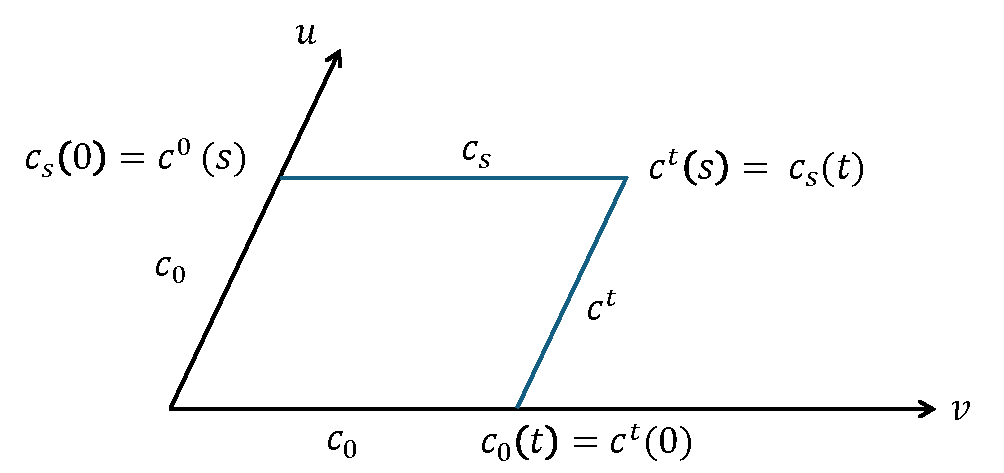
\includegraphics[width=0.5\textwidth]{graphics/parallelogram.pdf}
    \caption{Parallel transport around a parallelogram.}
\end{figure}
In Euclidean space, $P_{s,t} w = \operatorname{Id} w \forall s,t$. In general $P_{s,t}w - w \neq 0$.

\begin{lemma}
For $p \in M$ and $w \in T_pM$, the map
\[
\begin{aligned}
(-\epsilon, \epsilon) \times (-\delta, \delta) &\to T_pM \\
(s,t) &\mapsto P_{s,t}w
\end{aligned}
\]
is $C^{\infty}$ and satisifies
\[
\frac{\partial^2}{\partial s \partial t} P_{s,t}w\Bigg|_{(s,t)=(0,0)} = \lim_{(s,t)\to(0,0)}\frac{P_{s,t}w - w}{st},
\]
where the left-hand side is the Fréchet derivative for vector-valued functions.
Specifically, for an othonormal basis $e_1, \dots, e_n$ of $T_pM$,
\[
\frac{\partial^2}{\partial s \partial t} P_{s,t}w= \sum_{i=1}^n\left(\frac{\partial^2}{\partial s \partial t} \langle P_{s,t}w, e_i\rangle\right)e_i.
\]
\end{lemma}

\begin{proof}
Consider $s,t$ sufficiently small. Assume $\Im(c)$ is contained in a coordinate neighborhood $(U,\phi)$.
First, consider $P_{c_o(t)w}$. Let, 
\[
\phi(c_0(t)) = (c_0^1(t), \dots, c_0^n(t)),\quad P_{c_0(t)}w = \sum_{i=1}^n\xi^i(t)(\partial_i)_{c_0(t)},
\]
then $\xi^1(t), \dots, \xi^n(t)$ solve the linear ODE
\[
\frac{d\xi^k}{dt} + \sum_{i,j = 1}^{n}\Gamma_{ij}^k\frac{dc_0^i}{dt}\xi^j=0,\quad k=1,\dots,n,
\]
with initial condition $\sum_{i=1}^n \xi^i(0)(\partial_i)_p=w.$
Next, consider $P_{c^t(s)}P_{c_o(t)}w$. Let
\[
\sum_{i=1}^n \eta^i_t(s)(\partial_i)_{c^t(s)} = P_{c^t(s)}P_{c_0(t)}w.
\]
Then $\eta^1_t(s), \dots, \eta^n_t(s)$ solve the linear ODE
\[
\frac{d\eta^k_t}{ds} + \sum_{i,j = 1}^{n}\Gamma_{ij}^k\frac{d(c^t)^i}{ds}\eta^j_t=0,\quad k=1,\dots,n,
\]
with initial conditions $\eta_t^k(0) = \xi^k(t)$ ($k=1,\dots,n$).
By standard ODE theory, $\eta_t^k(s)$ are $C^{\infty}$ functions in $(s,t)$.
Repeating the same argument shows $P_{s,t}w$ is $C^{\infty}$ in $(s,t)$.

Fix an orthonormal basis $e_1, \dots, e_n$ of $T_pM$ and Taylor expand $\langle P_{s,t}w, e_i\rangle$ at $(s,t)=(0,0)$. Since 
$P_{s,0} = P_{0,t}w = w$,
\[
\frac{\partial^k}{\partial s^k}\langle P_{s,0},w,e_i\rangle = \frac{\partial^k}{\partial t^k}\langle P_{0,t}w,e_i\rangle = 0, \quad k\geq1.
\]
Then, $\forall i$,
\[
\langle P_{s,t}w,e_i\rangle = \langle w,e_i\rangle + st\frac{\partial^2}{\partial s\partial t}\langle P_{s,t}w, e_i\rangle\Bigg|_{(0,0)} 0 \mathcal{O}(st^2 + s^2t).
\]
It follows that
\[
\left\langle \lim_{(s,t)\to(0,0)}\frac{P_{s,t}w -w }{st},e_i\right\rangle = \frac{\partial^2}{\partial s\partial t}\langle P_{s,t}w,e_i\rangle\Bigg|_{(s,t)=(0,0)}.
\]
Multiplying by $e_i$ and summing over $i$ gives the desired result.
\end{proof}

\begin{definition}[Curvature tensor]
$\forall p \in M$, $u,v \in T_pM$, define $R(u,v) : T_pM \to T_pM$ by
\[
R(u,v)w := \frac{\partial^2}{\partial s \partial t} P_{s,t}w\Bigg|_{(s,t)=(0,0)} = \lim_{(s,t)\to(0,0)}\frac{P_{s,t}w - w}{st}, \quad w \in T_pM.
\]
The map $R:T_pM \times T_pM \times T_pM \to T_pM$ is called the \emph{curvature tensor}.
$R$ is a tensor field of type $(1,3)$.
\end{definition}

\begin{lemma}\label{lemma:8.3}
$\forall p \in M$ and $\forall w \in T_pM$, let $Z_{(s,t)} := P_{c^t(s)}P_{c_o(t)}w$. Then
\[
R(u,v)w = (\nabla_c + \nabla_{c_s}Z)\Big|_{(s,t)=(0,0)}.
\]
\end{lemma}

\begin{proof}
By \autoref{prop:covariant_derivative_along_curves_limit}, the covariant derivative along $c_s$ is 
\[
(\nabla_{c_s}Z)\Big|_{t=0} = \lim_{h\to0}\frac{P_{c_s(0)}Z(s,h) - Z(s,0)}{h}.
\]
Note that $c_0(h) = c^h(0)$ and $P_{c^h(0)}: T_{c^h(0)}M \to T_{c^h(0)}M$ is the identity map.
Since $P_{c_0(h)}: T_pM \to T_{c_0(h)}$ and $P_{c_0(0)}: T_{c_0(h)} \to T_pM$ are inverse to each other. We have
\[
\begin{aligned}
P_{c_0(0)}Z(s,h) &= P_{c_0(0)}P_{c^h(0)}P_{c_0(h)}w \\
&= P_{c_0(0)}P_{c_0(h)}w = w = Z(0,0).
\end{aligned}
\]
Consequently, $(\nabla_{c_s}Z)|_{(s,t)=(0,0)} = (\nabla_{c_0}Z)|_{t=0} = 0$.
Thus, the second covariant derivative satisifes
\[
\begin{aligned}
(\nabla_c + \nabla_{c^s}Z)|_{(s,t)=(0,0)} &= (\nabla_{c^0}\nabla_{c_s}Z)|_{s=0} \\
&= \lim_{k\to0}\frac{P_{c^0(0)}((\nabla_{c_s}Z)|_{(s,t)=(k,0)}) - (\nabla_{c_s}Z)|_{(s,t)=(0,0)}}{k} \\
&= \lim_{k\to0}\frac{P_{c^0(0)}\left(\lim_{h\to0}\frac{P_{c_k(0)}Z(k,h) - Z(k,0)}{h}\right)}{k} \\
&= \lim_{k\to0}\lim_{h\to0}\frac{P_{c^0(0)}\left(\frac{P_{c_k(0)}P_{c^h(k)}P_{c_0(h)}w - P_{c^0(k)}w}{h}\right)}{k} \\
&= \lim_{k\to0}\lim_{h\to0}\frac{P_{k,h}w-w}{hk} = R'.
\end{aligned}
\]
\end{proof}

\begin{definition}[Curvature tensor in coordinates]
On a coordinate chart of $M$, define
\[
R_{ijk}^l := \partial_i\Gamma_{jk}^l - \partial_j\Gamma_{ik}^l + \sum_{m=1}^n\left(\Gamma_{im}^l\Gamma_{jk}^m - \Gamma_{jm}^l\Gamma_{ik}^m\right)
\]
with $i,j,k,l = 1, \dots, n$.
\end{definition}

\begin{theorem}\label{thm:8.5}
$\forall p \in M$, $u,v,w \in T_pM$, let $u = \sum_{i = 1}^n u^i(\partial_i)_p$,
$v = \sum_{j=1}^n v^j(\partial_j)_p$ and $w = \sum_{k=1}^n w^k(\partial_k)_p$ in a chart. Then
\[
R(u,v)w = \sum_{i,j,k,l=1}^n u^iv^jw^kR_{ijk}^l(\partial_l)_p,
\]
multilinear in $u,v,w$. In particular, $R(u,v)w$ is independent of the choice of the chart.
\end{theorem}

\begin{proof}
Using notation from \autoref{lemma:8.3}, $Z$ is parallel along $c^t$. Thus,
\[
\nabla_{\partial/\partial s}^cZ = 0 \Rightarrow \nabla_{\partial/\partial t}^c\nabla_{\partial/\partial s}^cZ = 0.
\]
Since $\left[\frac{\partial}{\partial s}, \frac{\partial}{\partial t}\right]$, we have
\[
\begin{aligned}
&\left(\nabla_{\partial/\partial s}^c\nabla_{\partial/\partial t}^cZ - \nabla_{\partial/\partial t}^c\nabla_{\partial/\partial s}^cZ\right)\Big|_{(0,0)} \\
= &\left(\nabla_{\partial/\partial s}^c\nabla_{\partial/\partial t}^cZ \right)\Big|_{(0,0)} = (\nabla_{c^t}\nabla_{c_s}Z)|_{(0,0)} = R(u,v)w.
\end{aligned}
\]
The result follows by combining this with \autoref{prob:13}.
\end{proof}

\begin{problem}\label{prob:13}
Let $N$ be a manifold, $\xi : N\to M$ a $C^{\infty}$ map; $X,Y$ vector fields on $N$ and $Z$ a a vector field along $\xi$. 
In a coordinate chart of $M$, where
\[
d\xi(X) = \sum X^i\partial_i, \quad d\xi(Y) = \sum Y^j\partial_j, \quad Z = \sum Z^k\partial_k.
\]
Show that
\[
\nabla_X^{\xi}\nabla_Y^{\xi}Z - \nabla_Y^{\xi}\nabla_X^{\xi}Z = \sum_{i,j,k,l=1}^n X^iY^jZ^kR_{ijk}^l\partial_l.
\]
\end{problem}

The following follows from \autoref{prob:13}.

\begin{corollary}\label{cor:8.6}
\begin{enumerate}[label=(\arabic*), ref=Corollary \thecorollary~(\arabic*)]
\item \label{cor:8.6.1} For $\xi, X, Y, Z$ as in \autoref{prob:13},
\[
\nabla_X^{\xi}\nabla_Y^{\xi}Z - \nabla_Y^{\xi}\nabla_X^{\xi}Z - \nabla_{[X,Y]}^{\xi}Z = R(d\xi(X),d\xi(Y))Z.
\]
\item \label{cor:8.6.2} For vector fields $X,Y,Z$ on $M$
\[
R(X,Y)Z = \nabla_X\nabla_YZ - \nabla_Y\nabla_XZ - \nabla_{[X,Y]}Z.
\]
\end{enumerate}
Let $R_{ijkl} := \langle R(\partial_i,\partial_j)\partial_k, \partial_l\rangle$ be the coefficients of the $(0,4)$-tensor field.
By \autoref{thm:8.5},
\[
R_{ijkl} = \sum_{m=i}^nR{ijk}^mg_{ml}, \quad i,j,k,l=1,\dots,n.
\]
The fundamental symmetries of the cuvrature tensor are gievn in \autoref{prob:14}.
\end{corollary}

\begin{problem}\label{prob:14}
Show that $\forall p \in M, \quad u, v, w, x \in P_pM$ and indices $i,j,k,l$:
\begin{enumerate}[label=(\arabic*), ref=Problem \theproblem~(\arabic*)]
\item \label{prob:14.1} $R(u,v)w = -R(v,u)w$, $P_{jik}^l = -R_{ijk}^l$.
\item \label{prob:14.2} $R(u,v) + R(v,w) + R(w,u) = 0$.
\[
R_{ijk}^l + R_{jki}^l + R_{kij}^l = 0 \hfill \text{(first Bianchi identity)}.
\]
\item \label{prob:14.3} $\langle R(u,v)x, w \rangle = -\langle R(v,u)w, x \rangle$, $R_{ijkl} = -R_{jikl}$.
\item \label{prob:14.4} $\langle R(u,v)w, x \rangle = \langle R(x,x)u, v \rangle$, $R_{ijkl} = R_{klij}$.
\end{enumerate}
\end{problem}
\section{Sectional and Ricci curvatures}

Let $M$ be a Riemannian manifold.

\begin{lemma}\label{lemma:9.1}
$\forall p \in M$, let $\sigma \subset T_pM$ be a 2-dimensional subspace. For any basis $\{u,v\}$ of $\sigma$,
\[
K_{\sigma} := \frac{\langle R(u,v) u\rangle}{||u\times v||^2}
\]
is indendent of $\{u,v\}$, where
\[
||u\times v|| := \sqrt{||u||^2 ||v||^2 - \langle u,v\rangle^2}
\]
is the area of the parallelogram spanned by $u$, $v$.
\end{lemma}

\begin{proof}
Fix an orthonormal basis $\{e_1, e_2\}$ of $\sigma$ $\forall \{u,v\}$ basis of $\sigma$, let
\[
u = u^1e_1 + u^2 e_2, \quad v = v^1 e_1 + v^2 e_2.
\]
Then
\[
\begin{aligned}
\langle R(u,v)v, u\rangle &= \sum_{i,j,k,l=1,2}u^iv^ju^ku^l\langle R(e_i, e_j)e_k,e_l\rangle \\
&= [(u^1v^2)^2 + (u^2v^1)^2 - 2u^1u^2v^1v^2]\langle R(e_1,e_2)e_2,e_1\rangle \\
\Rightarrow \frac{\langle R(u,v)v, u\rangle}{||u\times v||^2} &= \langle R(e_1, e_2)e_2, e_1\rangle.
\end{aligned}
\]
\end{proof}

\begin{definition}[Sectional curvature]
$\forall o \in M$, $\forall \sigma \subset T_pM$ a 2-dimensional subspace and
$K_{\sigma}$ defined as in \autoref{lemma:9.1} is the \emph{sectional curvature}.
\end{definition}

\begin{remark}
The sectional curvature is undefined if $\dim M =1$. If $\dim M = 2$, $\sigma = T_pM$ $\Rightarrow K_{\sigma}$ is a function on $M$.
\end{remark}

\begin{theorem}[Sectional curvatures determine the Riemann curvature tensor]\label{theorem:9.3}
At each $p\in M$, the sectional curvatures
\[
\{K_{\sigma}|\sigma \subset T_pM \text{ is 2-dimensional}\}
\]
determine the Riemann curvature tensor $R$ at $p$.
\end{theorem}

\begin{proof}
$\forall u,v,w\in T_pM$, define 
\[
K(u,v) := \langle R(u,v)v,u\rangle, \quad R_w(u,v) := \langle R(u,w)w, v\rangle.
\]
If $\{u,v\}$ is linearly independednt $\Rightarrow K(u,v) = K_{\sigma} ||u\times v||^2$ for $\sigma = \operatorname{Span}_{\mathbb{R}}\{u,v\}$.
If $\{u,v\}$ is linearly dependent $\Rightarrow K(u,v) = 0$ by \autoref{prob:14}. 
Thus, sectional curvatures determine $K$.

$F_w$ is a symmetric bilinear form
\[
\begin{aligned}
F_w(u,v) &= \langle R(u,w)w, v\rangle\\
&= \langle R(w,v)u, w\rangle  \qquad\qquad {\text{\autoref{prob:14.4}}}\\
&= -\langle R(v, w)u, w\rangle \qquad\qquad {\text{\autoref{prob:14.1}}}\\ 
&= \langle R(v, w)w, u\rangle \qquad\qquad {\text{\autoref{prob:14.3}}}\\
&= F_w(v,w).
\end{aligned}
\]
Polarization yields
\[
\begin{aligned}
2F_w(u,v) &= F_w(u+v, u+v) - F_w(u, u) - F_w(v,v) \\
&= K(u+v, w) - K(u, w) - K(v, w).
\end{aligned}
\]
$K$ determines $F_W$. Expanding $R$ yields
\[
\begin{aligned}
R(u, v+w)(v + w) &= R(u, v)v + R(u, v)w + R(u, w)v + R(u, w)w \\
R(u+w, v)(u+w) &= R(u,v)u + R(u, v)w + R(w, u)u + R(w, v)w \\
&= R(u,v)w + R(v,u)w \\
R(u, v+w) - R(v,u+w)(u + w) &= 3R(u, v)w + R(u,v)v - R(v, u)u + R(u,w)w -R(v,w)w.
\end{aligned}
\]
Taking the inner product with $x \in T_pM$ and solving for $\langle R(u,v)w,x\rangle$:
\[
\begin{aligned}
\langle R(u,v)w, x\rangle &= \frac13\{F_{v+w}(u,x) + F_{u + w}(v,x) \\
& \qquad F_v(u,x) + F_u(u,x) \\
& \qquad - F_w(u,x) - F_w(v,x) \}.
\end{aligned}
\]
Thus, $R$ is uniquely determined by $K_{\sigma}$.
\end{proof}

\begin{corollary}\label{corollary:9.4}
$\forall p \in M$, the following are equivalent:
\begin{enumerate}[label=(\arabic*)]
\item $R(u,v)w = 0 \quad \forall u,v,w \in T_pM$.
\item $K_{\sigma} = 0 \quad \forall \text{ 2-dimensional } \sigma \subset T_pM$.
\end{enumerate}
\end{corollary}

\begin{definition}[Trace of a bilinear form]\label{def:9.5}
Let $V$ be an n-dimensional inner product space and $f:V\times V \to \mathbb{R}$ a bilinear form.
The \emph{trace} of $f$ is 
\[
\operatorname{tr} f := \sum_{i=1}^n f(e_i, e_i)
\]
where $\{e_1, \ldots, e_n\}$ is any orthonormal basis of $V$.
\end{definition}

\begin{remark}
Well-definedness (independence of $\{e_i\}_{i=1}^n$) is left as an exercise to the reader.
\end{remark}

\begin{definition}[Ricci and scalar curvature]\label{def:9.6}
$\forall p \in M$, $\forall v,w \in T_pM$, $\operatorname{Ric}(v,w)$ is the trace of the bilinear form
\[
\begin{aligned}
T_pM \times T_pM &\to \mathbb{R}, \\
(x,y) &\mapsto \langle R(x,v)w, y\rangle.
\end{aligned}
\]
For an orthonormal basis $\{e_1, \ldots, e_n\}$ of $T_pM$,
\[
\operatorname{Ric}(v,w) = \sum_{i=1}^n \langle R(e_i, v)w, e_i\rangle.
\]
The symmetric $(0,2)$-tensor $\operatorname{Ric}$ is the \emph{Ricci curvature tensor}.

For $v \in T_pM$ with $||v||=1$, $\operatorname{Ric}(v,v)$ is the \emph{Ricci curvature} 
in direction $v$. The trace of the Ricci tensor,
\[
\operatorname{Scal}(p) := \sum_{i=1}^n \operatorname{Ric}(e_i, e_i),
\]
is the \emph{scalar curvature} at $p$.
\end{definition}

\begin{proposition}
\label{prop:9.7}
$\forall v \in T_pM$ with $||v|| = 1$, let $\{e_1, \dots, e_n=v\}$ be an orthonormal basis of $T_pM$. 
Furthermore, let $\sigma_i \subset T_pM$ ($i = 1, \dots, n-1$) be the 2-dimensional subspace spanned by $\{e_i, v\}$ for $i=1, \ldots, n-1$. Then,
\[
\operatorname{Ric}(v,v) = \sum_{i=1}^{n-1} K_{\sigma_i}.
\]
\end{proposition}

\begin{remark}
If $\exists c \in \mathbb{R}$ such that $K_{\sigma} \geq c$ $\forall \sigma \text{ 2-dimensional subspace }\subset T_pM$ 2-dimensional $\Rightarrow \operatorname{Ric}(v,v) \geq (n-1)c$ $\forall \text{ unit vector } v \in T_pM$ (with $||v||=1$).
This is conventionally denoted as $\operatorname{Ric} \geq (n-1)c$.
\end{remark}


\section{Exponential maps}
Let $M$ be a Riemannian manifold for $p \in M$ and $v \in T_p M$, let $\gamma_v : J_v \to M$ be the maximal geodesic satisfying
$\gamma_v(0)  =p$ and $\gamma_v'(0) = v$, where $J_v$ is an open interval containing $0$.

\begin{definition}[Exponential map]
For $v \in TM$ if $1 \in J_v$, define $\exp v := \gamma_v(1)$.
Let $D:= {v \in TM | 1 \in J_v}$.
The map 
\[
\exp : D \to M
\]
is the \emph{exponential map}.
For $p \in M$, let $D_p := D \cap T_pM$. The map
\[
\begin{aligned}
    &\exp_p : D_p \to M \\
    &\exp_p := \exp|_{D_p},
\end{aligned}
\]
is the \emph{exponential map} at $p$.

$\exp_p v \quad (v \in T_pM)$ is the point reached by traveling along the geodesic from $p$ in direction $v$ for the distance $\|v\|$.
$\forall v \in D_p$ and $0 \leq \forall t \leq 1$ $1 \in J_v = t J_{tv} \subset J_{tv} \implies tv \in D_p$.
Thus, $D_p$ is a star shaped domain.
\end{definition}

\begin{proposition}
    $D \subset TM$ and $D_p \subset T_p M$ are open.
    Both $\exp$ and $\exp_p$ are $C^{\infty}$
    \label{prop:10.2}
\end{proposition}
\begin{proof}
Follows from \autoref{prop:7.10}.
\end{proof}

Let $0_p$ denote the zero vector in $T_p M$.
\begin{proposition}[The differential map]
    $d(\exp_p)_{0_p} : T_{0_p} T_p M \approx T_p M \to T_p M$ is the identity.
    \label{prop:10.3}
\end{proposition}

\begin{proof}
    For $v \in T_p M$, let $c(t) := tv$. Then $(\exp_p \circ c)(t) = \exp_p(tv) = \gamma_v(t)$.
    This shows that: 
    \[
    \begin{aligned}
        d \exp_p(v) &= d \exp_p (c'(0))= (\exp_p \circ c)'(0) \\
        &= \gamma_v'(0) = v 
    \end{aligned}
    \]
\end{proof}

Let $\pi : TM \to M$ be the natural projection.

\begin{lemma}
    Define $f: D \to M \times M$ by
    \[
    \begin{aligned}
        \exp f(v) := \left( \pi(v), \exp v\right), v \in D
    \end{aligned}
    \]
    $\forall p_0 \in M$, $\exists$ open neighbourhood $0_{p_0} \subset TM$ of $0_{p_0}$ such that
    \begin{enumerate}
        \item $0_{p_0} \subset D$
        \item $\exp f(0_{p_0})$ is open in $M \times M$
        \item $\exp f : 0_{p_0} \to \exp f(0_{p_0})$ is a diffeo.
    \end{enumerate}
    \label{lemma:10.4}
\end{lemma}

\begin{proof}
    Fix chart $(U, \phi)$ aroun $p_0$ $\implies$ induced chart $(TU,\tilde{\phi})$ for $TM$. let:
    $\tilde{\phi}(v) = (x^1, \dots, x^n, v^1, \dots, v^n)$.
    $\phi(\exp v) = (y^1, \dots, y^n)$.
    Local expression $\bar{f} := (\phi \times \phi) \circ \exp f \circ \tilde{\phi}^{-1}$ is:
    \[
    (f^1, \dots, f^{2n}) := \bar{f}(x^1, \dots, x^n, v^1, \dots, v^n) = (x^1, \dots, x^n, y^1, \dots, y^n)
    \]
    Jacobian of $\bar{f}$ at $(\phi(p_0),0)$ is non-singular.
    By Inverse Function Theorem, $\exists$ open $0 \subset \mathbb{R}^{2n}$ such that
    $\bar{f}|_0$ is a diffeo and $\bar{f}(0)$ is open/
    Set $0_{p_0} := \tilde{\phi}^{-1}(0)$
\end{proof}

\begin{problem}
    Provide details for Proof of \autoref{lemma:10.4}.
    Specifically, show non-singularity of Jacobian of $\bar{f}$ at 
    $(x^1, \dots, x^nm v^1, \dots, v^n) = (\phi(p_0),0. \dots,0)$. 
    \label{problem:10.5}
\end{problem}

\begin{lemma}\label{lemma:10.5}
    $\forall p_0 \in M$, $\exists$ open neighbourhood $0$ of $p_0, \quad \exists r >0$ such that $\forall p \in 0$:
    \begin{enumerate}
        \item $B(0_p,r) \subset D_p$
        \item $\exp_p (B(0_p,r))$ is open in $M$
        \item $\exp_p : B(0_p,r) \to \exp_p(B(0_p,r))$ is a diffeo.
    \end{enumerate}
    Here $B(0_p,r) \subset T_p M$ is the open ball of radius $r$ centered at $0_p$.
\end{lemma}
\begin{proof}
    Let $f: 0_{p_0} \to f(0_{p_0})$ be the diffeo from \autoref{lemma:10.4}, since $0_{p_0}$ is an open neighbourhood of $0_{p_0}$,
    $\exists O \subset M$: open around $p_0$ such that $r>0$ such that
    \[
    TO(r) := {v \in TM | \pi(v) \in O, |v| <r} \subset 0_{p_0}
    \]
    $\forall p \in O$, $B(0_p,r) \subset TO(r) \subset 0_{p_0} \subset D \implies (1)$ holds.
    Define $Q_P := {q \in M| (p,q) \in f(0_{p_0})}$
    Since $f(0_{p_0}) \subset M \times M$ is open, $Q_p$ is also open.

    \[
\left(
\begin{array}{c@{\;}c@{\;}c@{\;}c}
    h \colon & M & \to & M \times M \\
    & \rotatebox[origin=c]{90}{$\in$} & & \rotatebox[origin=c]{90}{$\in$} \\
    & q & \mapsto & (p, q)
\end{array}
\text{ is continuous and } Q_p = h^{-1}(f(O_{p_0})).
\right)
\]
The inverse
\[
f^{-1}(p,q)  = \exp_p^{-1}(q), \quad (p,q) \in f(0_{p_0})
\]
is $C^{\infty}$, so $\exp_p^{-1}\|_{Q_p} : Q_p \to T_p M \cap 0_{p_0}$ is $C^{\infty}$ for fixed $p$.
Thus $\exp_p: T_p M \cap 0_{p_0} \to Q_p$ is a diffeomorphism. Since $B(0_p,r) \subset 0_{p_0}$, (2) and (3) follow.
\end{proof}

\begin{theorem}[Gauss Lemma]
    $\forall p \in M$ and $\forall v,w \in T_pM$, the following hold:
    \begin{enumerate}
        \item $d(\exp_p)_v v = \gamma_v'(1)$
        \item $\langle \gamma_v'(1), d(\exp_p)_v w \rangle = \langle v, w \rangle$.
    \end{enumerate}
    Here, $w$ is identified with a vector at $v \in T_pM$ via $T_pM \approx T_v T_pM$
    \label{theorem:10.6}
\end{theorem}

\begin{proof}
\begin{enumerate}[label=(\arabic*)]
\item follows from $\gamma_v'(1) = \frac{d}{dt} \exp_p (tv) |_{t=1}= d(\exp_p)_v v$.

\item Let $ p \in M$ and $v,w \in T_pM$. Case $v=0_p$ is trivial.
Assume $ v \neq 0_p$. consider variation:
\[
\begin{aligned}
&c_s (t) := c(s,t) := \exp_p (t(v+sw)), \quad s \in (- \epsilon, \epsilon), 0 \leq t \leq 1. \\
&c_0(t) = \exp_p (tv) = \gamma_v (t) \text{ is a geodesic}
\end{aligned}
\]
$\implies \nabla_{c_0} = 0$. Variation field $X(t) = d(\exp_p)$.
By 1st variation formula (cf. \autoref{theorem:7.2})
\[
\begin{aligned}
\frac{d}{ds} L(C_s)|_{s=0} &= \frac{1}{|c_0'(0)|} \left( \langle c_0'(1, X(1)) \rangle - \langle c_0'(0), X(0) (=0) \rangle \right) \\
&= \frac{1}{|v|} \langle \gamma_v'(1), d(\exp_p)_v(w) \rangle
\end{aligned}
\]
Alternativly, $L(Cs) = |v+sw| = \langle v+sw, v +sw \rangle^{1/2}$
\[
\frac{d}{ds} L(Cs) |_{s=0} = \frac{\langle \frac{d}{ds}(v+sw), v +sw \rangle|_{s=0}}{|v|} = \frac{\langle v,w \rangle}{|v|}
\]
\end{enumerate}
\end{proof}

\begin{remark}
    Combining (1) and (2) yields:
    $$
    \langle d(\exp_p)_v v, d(\exp_p)_v w \rangle = \langle v,w \rangle
    $$
    Thus, Gauss Lemma is weaker than $d(\exp_p)v$ being isometric.
    If ${v,w}$ is linearly dependent $|d(\exp_p)_v w | = |w|$.
    In general $d(\exp_p)_v$ is not isometric.
    For example, $M = \mathbb{S}^2 \subset \mathbb{R}^3, \quad v \in T_pM; \|v\|=\pi$.
    $d(\exp_p)_v$ is an isometry $\implies$ it is injective.
    By the inverse function theorem, $\exp_p$ is a diffeo on a neighbourhood of $v$. However, this is impossible since for $\forall v' \in T_pM$ satisfying 
    $\|v'\| = \pi, \quad \exp_p v'$ coincides with the antipodal point of $p$.
    \label{remark:10.7}
\end{remark}

\begin{lemma}\label{lemma:10.8}
$\forall p \in M$, $\forall v \in T_pM$, let $\sigma : [0,l]\to D_p$ be a piecewise smooth regular curve s.t. $\sigma(0)  0_p$ and
$\sigma(l)= v$. Then
\[
L(\exp_p \odot sigma) \geq ||v||.
\]
furthemore, if $d(\exp_p)_{\sigma(t)}$ is non-singular $\forall t \in [0,l]$, then
for every monotonically increasing function $f:[0,l] \to [0,1]$ with $f(0) = 0, f(l) = 1$,
\[
\sigma(t) = f(t)v.
\]
\end{lemma}

\begin{proof}
Assume $v \neq 0$. Let 
\[
t_0 := \sup\{t \in [0,l] : \sigma(t) = 0_p\}.
\]
$\forall t \in (t_0, l)$, let $r(t) := ||\sigma(t)|| >0$ and $e(t) \in t_pM$ be the unit vector s.t. $\sigma(t) = r(t)e(t)$.
Let also $c(t):= \exp_p \odot \sigma(t)$. Since $\sigma'(t) = r'(t)e(t) + r(t)e'(t)$, 
\[
\begin{aligned}
c'(t) &= d(\exp_p)_{\sigma(t)}\sigma'(t) \\
&= r'(t) d(\exp_p)_{\sigma(t)}e(t) + r(t)d(\exp_p)_{\sigma(t)}e'(t) \\
&= \frac{r'(t)}{r(t)}\gamma'_{\sigma(t)}(1) + r(t)d(\exp_p)_{\sigma(t)}e'(t).
\end{aligned}
\]
By Gauss' lemma,
\[
\begin{aligned}
\langle \gamma'_{\sigma(t)}(1),d(\exp_p)_{\sigma(t)}e'(t)\rangle &= r(t) \langle e(t), e'(t)\rangle \\
&= \frac{r(t)}{2} \frac{d}{dt} \langle e(t), e(t) \rangle = 0.
\end{aligned}
\]
Thus the decomposition of $c'(t)$ above is an orthogonal decomposition.
Since $|\gamma'_{\sigma(t)}(1)| = ||\sigma(t)|| = r(t)$, we have
\[
|c'(t)| = \sqrt{|r'(t)|^2 + ||r(t)d(\exp_p)_{\sigma(t)}e'(t)||^2} \geq |r'(t)| \geq r'(t).
\]
Integrating gives
\[
\begin{aligned}
L(c|_{[t_0,l]}) &= \int_{t_0}^l|c'(t)|dt \geq \int_{t_0}^lr'(t)dt \\
&= ||\sigma(l)|| - ||\sigma(t_0)|| = ||\sigma(l)|| = ||v||.
\end{aligned}
\]
This proves $L(\exp_p\odot\sigma) \geq ||v||$.

Now assume $d(\exp_p\odot\sigma)$ is non-singular and $L(\exp_p\odot\sigma)= ||v||$. Then the above inequality implies that 
$L(\exp_p\odot\sigma|_{[0,t_0]}) = 0 \Rightarrow \sigma(t) = 0_p$ on $[0,t_0]$.
This implies
\[
|c'(t)| = |r'(t)| = r'(t).
\]
Thus, the second term in the othogonal expansion of $c'(t)$ must vanish, i.e. $d(\exp_p)_{\sigma(t)}e'(t) = 0$.
Since $d(\exp_p)_{\sigma(t)}$ is non-singular, $e'(t) = 0_p$, implying that $e(t)$ is constant. So
\[
e(t) = e(l) = v/||v||.
\]
Setting $f(t) := r(t)/||v||$ yields $\sigma(t)=f(t)v$.
\end{proof}

\begin{lemma}\label{lemma:10.9}
Let $p \in M$, $r>0$. Assume $B(0_p,r) \subset D_p$ and $\exp_p : B(0_p,r) \to \exp_p(B(0_p,r))$ is a diffeoorphism.
Then
\begin{enumerate}[label=(\arabic*)]
\item $\forall q \in \exp_p(B(0_p,r))$, $\exists ! v \in B(0_p,r)$ s.t. $q = \exp_pv$.
Any piecewise smooth minimizing curve connecting $p$ and $q$ coincides with the geodesic $\gamma_v : [0,1] \to <$ up to
reparametrization.
\item $\exp_p(B(0_p,r)) = B(p,r)$.
\end{enumerate}
\end{lemma}

\begin{proof}
\begin{enumerate}[label=(\arabic*)]
\item Existence and uniqueness of $v$ follows from the bijectivity of $\exp_p$.
Let $c:[0,1] \to M$ be a piecewise smooth curve from $p$ to $q$. Define
\[
\sigma(t) := (\exp_p|_{B(0_p,r)})^{-1}\odot c(t),
\]
whenever $c(t) \in \exp_p(B(0_p,r))$.
\begin{enumerate}[label=(\roman*)]
\item If $c([0,1]) \not\subset \exp_p(B(0_p,r))$: Let $0<\rho < r$.
Define $l := \sup\{t\in[0,1]:c([0,t)\subset\exp_p(B(0_p,\rho))\}$.
set $U := \exp_p(B(0_p,\rho))$ and $\phi := (\exp_p|_{B(0_p,\rho)})^{-1}:U \to B(0_p,\rho)$ and
identiy $T_pM \approx \mathbb{R}^n$. Applying \autoref{lemma:1.16} to $(U,\phi)$ it follows that
$\sigma(l) \in \partial B(0_p,\rho)$ since $\sigma(l) \notin B0_p,\rho)$. % I think Lemma 1.16 in his notes is 1.23 in our notes.
By \autoref{lemma:10.8}, we have 
\[
L(c) \geq L(c|_{[0,l]}) \geq ||\sigma(l)|| = \rho.
\]
Since $\rho$ was arbitrary, $L(c) \geq r$. However, $L(\gamma_v|_{[0,1]}) = ||v|| < r$. Thus,
\[
L(\gamma_v)_{[0,1]} < r \leq L(c).
\]
\item If $c([0,1])\subset\exp_p(B(0_p,r))$: $\sigma(t)$ is defined $\forall t \in [0,1]$.
By \autoref{lemma:10.8}, $L(c) \geq ||v|| = L(\gamma_v|_{[0,1]})$.
\end{enumerate}
In both cases, $L(c) \geq L(\gamma_v|_{[0,1]})$, so $\gamma_v$ is a minimizing curve
connecting $p$ and $q$. Then, $L(\gamma_v|_{[0,1]}) = L(c)$. In this case, if $c([0,1]) \not\subset\exp_p(B(0_p,r))$, then by
(i), we have $L(\gamma_v)_{[0,1]} < L(c)$, which is a contradiction. Therefore, $c([0,1]) \subset \exp_p(B(0_p,r))$. 
Furthermore, by the last part of \autoref{lemma:10.8}, there exists a non-decreasing function $f:[0,1]\to[0,1]$ s.t.
\[
f(0)=0,\quad f(1)=1, \quad \sigma(t) = f(t)v\quad \text{ for } t \in [0,1].
\]
Thus, by reparametrizing $c$ as $\tilde{c}(t) := (c\odot f^{-1})$, we have 
\[
\tilde{c}(t) = c(f^{-1}(t)) = \exp_p(f(f^{-1}(t))v) = \exp_p(tv) = \gamma_v(t).
\]
\item For $q \in \exp_p(B(0_p,r))$, let $q=\exp_p$.
Since $\gamma_v$ is minimizing,
\[
d(p,q) = L(\gamma_v) = ||v|| < r \Rightarrow q \in B(p,r).
\]
Conversely, let $q \in B(p,r) \Rightarrow d(p,q) < r$. Then, there exists a curve $c$ connecting $p$ and $q$ s.t. $L(c) <r$.
If $c([0,1]) \not\subset \exp_p(B(0_p,r))$, by (1i), $r \leq r$, a contradiction.
Thus $c([0,1]) \subset \exp_p(B(0_p,r))$, specifically $q \in \exp_p(B(0_p,r))$.
\end{enumerate}
\end{proof}

Combining \autoref{lemma:10.5} and \autoref{lemma:10.9}, we have the following:

\begin{theorem}\label{theorem:10.10}
$\forall p_0 \in M$, there exists an open neighbourhood $0 \subset M$ of $p_0$ and $r >0$ s.t. the following hold
\begin{enumerate}[label=(\arabic*)]
\item $\forall p \in 0$, $B(0_p,r) \subset D_p$ and $\exp_p:B(0_p,r)\to B(p,r)$ is a diffeomorphism.
\item $\forall p \in 0$ and $\forall q \in B(p,r)$, there exists a unique piecewise smooth minimizing curve
(up to renormalization) connecting $p$ and $q$. Thus curve is the geodesic $\gamma_v:[0,1]\to M$ where
\[
v = (\exp_p|_{B(0_p,r)})^{-1}(q) \in B(0_p,r).
\]
\end{enumerate}
\end{theorem}
A piecewise smooth regular curve $c : (a,b) \to M$ is locally minimizing if and only if $\forall t_0 \in (a,b)$,
$\exists \delta > 0$ s.t. $[t_0 - \delta, t_0 + \delta] \subset (a,b)$ and $c|_{[t_0 - \delta, t_0 + \delta]}$
is the minimizing curve between $c(t_0 - \delta)$ and $c(t_0 + \delta)$.
Sub-arcs of minimizing curves are themselves minimizing, in particular every minimizing curve is locally minimizing (verify this yourself).

\begin{theorem}\label{theorem:10.11}
Let $\gamma:(a,b) \to M$ be a piecewise smooth regular curve. Then
\[
\gamma \text{ is a geodesic} \Leftrightarrow \gamma \text{ is locally minimizing}.
\]
\end{theorem}

\begin{proof}
($\Rightarrow$): $\forall t_0 \in (a,b)$, let $p_0:=\gamma(t_0)$. Apply \autoref{theorem:10.10} to get $0$ and $r>0$.
Choose $\delta >0$ s.t. $\gamma < r/2$, $[t_0-\delta,t_0+\delta]\subset(a,b)$ ane $\gamma(t_0-\delta) \in 0$.
Since $L(\gamma|_{[t_0-\delta,t_0+\delta]})=2\delta < r$, $\gamma([t_0-\delta,t_0+\delta])\subset B(\gamma(t_0-\delta),r)$.
By \autoref{theorem:10.10}, for $p:=\gamma(t_0-\delta)$ and $q := \gamma(t_0+\delta)$, the curve $\gamma|_{[t_0-\delta,t_0+\delta]}$ is minimizing.
Thus $\gamma$ is locally minimizing.

($\Leftarrow$): Let $t_0 \in (a,b)$, $\delta' >0$ s.t. $\gamma|_{[t_0-\delta',t_0+2\delta']}$ is minimizing.
Apply \autoref{theorem:10.10} at $p_0 := \gamma(t_0)$ to get $0$ and $r>0$.
Choose $\delta >0$ s.t. $\delta \leq \delta'$, $\delta < r/2$ and $r(t_0 - \delta) \in 0$.
let $p:= \gamma(t_0 - \delta)$, $g := \gamma(t_0 + \delta)$. Since $\delta \leq \delta'$,
$\gamma|_{[t_0-\delta,t_0+\delta]}$ is minimizing between $p$ and $q$. since $d(p,q) = d\delta <r$, \autoref{theorem:10.10} (2) implies that
$\gamma|_{[t_0-\delta,t_0+\delta]}$ is a geodesic.
Since $t_0$ was arbitrary, $\gamma$ is a geodesic.
\end{proof}

\begin{definition}[Normal neighbourhood and coordinates]
assume $\exp_p:B(0_p,r) \to B(p,r)$ is a diffeomorphism for $p \in M$ and $r >0$. Let $\{e_i\}$ be an 
orthonormal basis of $T_pM$. For $q \in B(p,r)$, define
\[
x^i := \langle (\exp_p|_{B(0_p,r)})^{-1},e_i\rangle, \qquad (i=1,\dots,n),
\]
so that $q = \exp_p\left(\sum_{i=1}^n x^i e_i\right)$. The coordinates $\phi(q) = (x^1,\dots,x^n)$ defines a coordinate chart $(B(p,r),\phi)$.
this is the \emph{normal coordinate neighbourhood} at $p$ subordinated to $\{e_i\}$ and $(x^1,\dots,x^n)$ are \emph{normal coordinates}.
\end{definition}

The following is a consequence of \autoref{theorem:10.10}:

\begin{corollary}
$\forall p \in M$, normal coordinate neighbourhood exists around $p$.
\end{corollary}

Let $\{e_i\}$ be an orthonormal basis of $T_pM$, $(x^1,\dots,x^n)$, the subordinated normal coordinates at $p$ and $E_i := \partial/\partial x^i$.
\begin{problem}\label{problem:16}
Show that $\forall i,j,k = 1,\dots,n$:
\begin{enumerate}[label=(\arabic*)]
\item $(E_i)_p = e_i$,
\item $\nabla_{e_i}E_j = 0$ and $\Gamma_{ij}^k(p) = 0$.
\end{enumerate}
\end{problem}

\begin{remark}
The equlities is \autoref{problem:16} hold only at a specific point $p$.
\end{remark}
\section{Completeness and the Hopf-Rinow Theorem}

\begin{definition}[Geodesically completeness]
    $M$ is geodesically complete $: \equiv$ the domain of every geodesic can be extended to $mathbb{R}$ (i.e. $Ju = \mathbb{R}$).
    Alternativly, $M$ is a geodesically complete $\equiv$ $exp_p$ is defines on $T_pM$ (i.e. $D_p = T_pM$) $\forall p \in M$.
    We will prove that if $M$ is a geodesically complete Riemannian manifold, any two points in $M$ ccan be connected by a minimizing geodesic.
    \label{def:11.1}
\end{definition}

\begin{lemma}
    Let $M$ be geodesically complete.
    For $p \in M$, by \autoref{theorem:10.10}, $\exists r >0$ s.t.
    $exp_p : B(0_p, r) \to B(p,r)$ is a diffeo and there exists a unique minimizing geodesic from $p$ to any point in $B(p,r)$.
    For $\rho \in \mathbb{R}$ with $0<\rho<r$, any $g \in M \backslash  B(p,p)$
    admits $\hat{p} \in \partial B(p,p)$ s.t. $\rho + d(\hat{p}, q) = d(p,q)$
    \label{lemma:11.2}
\end{lemma}

\begin{proof}
    $\partial B(p,p)= exp_p (\partial B(0_p,p))$ is cpt.
    Since $f(x) := d(q,x)$ is continous (cf. \autoref{prop:open_in_manifold}),
    $f$ attains a minimum on $\partial B(p,p)$. Let $\hat{p} \in \partial B(p,p)$
    be the minimizer. By the triangle inequality:
    \[
    \begin{aligned}
        \rho + d(\hat{p}, q) = d(p,\hat{p}) + d(\hat{p},q) \geq d(p,q)
    \end{aligned}
    \]
    Conversly, let $c:[0,l] \to M$ be a piecewise smooth regular curve from $p$ to $q$. By definition: $d(p,q) = \inf_c L(c)$.
    $h(t) := d(p, c(t))$ is continous with $h(0) =0$ and $h(l) = d(p,q) \geq p$
    By the intermediate value theorem, $\exists t_0 \in [0,l]$ s.t. $d(p,c(t_0)) = \rho$. Then:
    \[
    \begin{aligned}
        L(c) &= L(c|_{[0,t_0]}) + L(c|_{t_0,l}) \\
        &\geq d(p,c(t_0)) + d(c(t_0),q) \geq \rho + d(\hat{p},q)
    \end{aligned}
    \]
    Taking inf. over $c$: $d(p,q) \geq \rho + d(\hat{p}, q)$
\end{proof}

\begin{theorem}
    Assume $p \in M$ and $exp_p$ is defined on the entire $T_pM$. Then, $\forall q \in M$, there exists a minimizing geodesic containing $p$ and $q$.
    In pparticular, if $M$ is geodesically complete, any two points in $M$ can be connected by a minimizing geodesic.
    \label{theorem:11.3}
\end{theorem}

\begin{proof}
    fix $r>0$ and $0 < \rho <r$ for $p \in M$ as in \autoref{lemma:11.2}.
    Assume $q \notin B(p,p)$ by taking a smaller $\rho$ if necessary.
    By \autoref{lemma:11.2}, $\exists \hat{p} \in \partial B(p,\rho)$ such that $p+ d(\hat{p},q) = d(p,q)$.
    By \autoref{theorem:10.10}, $\exists v \in T_pM \quad (\|v\| =1)$ such that
    $\gamma_v (d(p,\hat{p})) = \hat{p}$ and $\gamma_v |_{[0,d(p,\hat{p})]}$ is a minimizing geodesic.
    We show $\gamma_v |_{[o,d(p,q)]}$ is the minimzing geodesic from $p$ to $q$.

    Define $T := {t \in [0,d(p,q)]|\gamma_v |_{[0,t]} \text{ is a minimizing geodesic and } t+d(\gamma_v(t),q) = d(p,q)}$
    Then $\rho \in T$. since $T$ is a bounded closed set, it has a maximum element $t_{max}$. Assume $t_{max} < d(p,q)$.
    For $p_1 := \gamma_v (t_{max})$, fix $r_1 > 0$ and $0<\rho_1 <r_1$ as in \autoref{lemma:11.2}, assuming $q \notin B(p_1, \rho_1)$
    Then $\exists \hat{p}_1 \in \partial B(p_1, \rho_1)$ such that
    \[
    \begin{aligned}
        \rho_1 + d(\hat{p}_1,q) = d(p_1,q).
    \end{aligned}
    \]
    Since $t_{max} \in T$,
    \[
    \begin{aligned}
        d(p,\rho_1) + d(\rho_1,q) = d(p,q).
    \end{aligned}
    \]
    Combining these:
    \[
    \begin{aligned}
        d(p,p_1) + \rho_1 + d(\hat{p}_1,q) = d(p,q)
    \end{aligned}
    \]
    By the triangle inequality $d(p,q) \leq d(p, \hat{p}_1) + d(\hat{p}_1,q)$ and \autoref{def:11.1} $d(p, \hat{p}_1) \geq d(p, p_1) + \rho_1$
    Let $\sigma$ be the minimizing geodesic from $p_1$ to $\hat{p}_1$, so $L(\sigma) = \rho_1$. Yje triangle inequality yields the reverse inequality.
    Thus $d(p, \hat{p}_1) = d(p,p_1) + \rho_1 = L(\gamma_v|_{0,t_{max}})+L(\sigma)$.
    The concatenated curve of $\gamma_v |_{[0, t_{max}]}$ and $\sigma$ connects $p$ and $\hat{p}_1$ with length $d(p, \hat{p}_1)$, hence it is a minimizing curve.
    Being locally minimizing, it is a geodesic by \autoref{theorem:10.11} and coincides with $\gamma_v |_{[0,t_{max}+\rho_1]}$. With \autoref{def:11.1},
    $t_{max} + \rho_1 \in T$, contradicting the maximality of $t_{max}$.
    Thus $t_{max}=d(p,q)$, implying:
    \[
    \begin{aligned}
        &d(p,q) + d(\gamma_v(t_{max}),q) = d(p,q) \\
        &\implies \gamma_v (d(p,q)) =q
    \end{aligned}
    \]  
\end{proof}
 
\begin{problem}
    In the proof of \autoref{theorem:11.3}, show that $T$ is a closed set.
    In a metric space $(X,d)$, $(X,d)$ is said to be complete $: \equiv \forall$ Cauchy sequences is a convergent sequence.
    A subset $A \subset X$ is bounded $: \equiv \sup_{p,q \in A} d(p,q) < + \infty$
\end{problem}

\begin{theorem}[Hopf-Rinow Theorem]
    The following are equivalent:
    \begin{enumerate}
        \item $M$ is a geodesically complete
        \item $\forall$ bounded closed subset of $M$ is cpt
        \item $(M,d)$ is a complete metric space with respect to Riemannian distance $d$
    \end{enumerate}
    \label{theorem:11.4}
\end{theorem}

\begin{proof}
    $(1) \implies (2)$: $\forall$ bounded closed set $C \subset M$.
    $\exists r>0$ such that $C \subset B(,r)$. Since $\bar{B}(0_p,r)\subset T_pM$ is cpt and $exp_p: T_p M \to M$ is continous, the image
    $\bar{B}(p,r) = exp_p (\bar{B}(0_p,r))$ is cpt.
    Since $C$ is a closed subset of a cpt set, $C$ is cpt.
    $(2) \implies (3):$ Let ${p_i}^{\infty}_{i=1}$ be a cauchy sequence $\exists i_1 \in \mathbb{N}$ such that $d(p_i, p_j) < 1$ $\forall i,j \geq i_1$ Setting
    \[
    \begin{aligned}
        R := \max_{i=1, \dots, i_1} d(p_1,p_i) +1,
    \end{aligned}
    \]
    the triangle inequality implies that $\forall i > i_1$, we have 
    \[
    \begin{aligned}
        d(p_1, p_i) \leq d(p_1, p_{i1}) + d(p_{i1},p_i) < R
    \end{aligned}
    \]
    thus we have $d(p_1,p_i) < R$ $\forall i \in \mathbb{N}.$
    Hence ${p_i} \subset \bar{B}(p_1,R)$ which is cpt by $(2)$.
    $\exists$ subsequence ${p_{j(i)}}$ such that $p:= \lim_{i \to \infty} p_{j(i)} \in \bar{B}(p_1,R)$.
    $\forall \epsilon >0$, since ${p_i}$ is Cauchy, $\exists i_{\epsilon} \in \mathbb{N}$ such that $d(p_i, p_j) < \frac{\epsilon}{2}, \quad \forall i,j \geq i_{\epsilon}$
    Take $i' \in \mathbb{N}$ sufficiently large so that $j(i') \geq i_{\epsilon}$ and $d(p_{j(i')},p) < \frac{\epsilon}{2}.$
    Then $\forall i \geq i_{\epsilon}$, we obtain:
    \[
    \begin{aligned}
        d(p_i,p) \leq d(p_i, p_{j(i')}) + d(p_{j(i')},p) < \epsilon
    \end{aligned}
    \]
    Thus $\lim_{i \to \infty} p_i = p$.
    $(3) \implies (1)$: Fix $p \in M$, $v \in T_p M \quad (\|v\| = 1)$
    Suppose $t_0 := \sup {t>0 | tv \in D_p} < + \infty$
    Since $D_p$ is open, $t_ov \notin D_p$.
    For $t_i \to t_0$, $d(\gamma_v (t_i), \gamma_v(t_j)) \leq |t_j - t_i |$
    implies ${\gamma_v (t_i)}$ is Cauchy. By $(3)$, $\gamma_v (t_1) \to \exists p_0 \in M$
    as $i \to \infty$, which contradicts \autoref{prop:7.9}
\end{proof}

In the proof $(1) \implies (2)$ of \autoref{theorem:11.4} the choice of $r>0$ is determined by the bounded set $C$, and no specific
properties of the map $exp_p : B(0_p,r) \to exp_p (B(0_p,r))$ are assumed. Consequently, (11.2) is non-trivial.

\begin{problem}
    Prove \autoref{lemma:11.2}. Furthermore, provide an example where \autoref{lemma:11.2} fails when $M$ is not geodesically complete.
    If $M$ is geodesically copmlete ($\equiv$ the Riemannian distance is complete),
    we simply say $M$ is complete.
\end{problem}

\begin{theorem}[Remember]
    Geodesic completeness of $M$ does not imply that every $C^{\infty}$ vector field on $M$ is complete.
    In fact, recall: $\forall c^{\infty}$ v.f. on $M$ is complete $\equiv$ $M$ is cpt.
\end{theorem}
\section{Jacobi fields}

Let $M$ be a $n$-dimensional Riemannian maifold and $\gamma:[0,l]\to M$ a geodesic.

\begin{definition}[Jacobi field and Jacobi equation]\label{def:12.1}
A vector field $J(t)$ along $\gamma$ is a \emph{Jacobi field}
if it satisifies
\[
(\nabla_{\gamma}\nabla_{\gamma}J)(t) + R(J(t),\gamma'(t))\gamma'(t) = 0, \quad t \in [0,l]
\]
This is called the \emph{Jacobi equation}.
\end{definition}

Fix $t_0 \in [0,l]$ and an orthonormal basis $e_1, \dots, e_n$ of $T_{\gamma(t_0)}M$.
Let $E_i(t)$ be parallel vector field along $\gamma$ such that
$E_i(t_0) = e_i$. Then $E_1(t), \dots E_n(t)$ is an orthonormal basis of $T_{\gamma(t)}M$ for all $t \in [0,l]$.
For any vector field $J(t)$ along $\gamma$, let
\[
\begin{aligned}
J(t) &= \sum_{i=1}^nJ^i(t) E_i(t), \\
(\nabla_{\gamma}\nabla_{\gamma}J)(t) &= \sum_{i=1}^n(J^i)''(t)E_i(t), \\
R(J(t), \gamma'(t))\gamma'(t) &= \sum_{j=1}^nJ^i(t) R(E_j(t), \gamma'(t))\gamma'(t) \\
&= \sum_{j=1}^n\sum_{i=1}^nJ^j(t)\langle R(E_j(t), \gamma'(t))\gamma'(t), E_i(t)\rangle E_i(t) \\
&= \sum_{i=1}^n\left(\sum_{j=1}^n J^i(t)R_{ij}(t)\right)E_i(t),
\end{aligned}
\]
where $R_{ji}(t) = R_{ij}(t)$ has been used. Define
\[
\vec{J}(t) := (J^1(t), \dots, J^n(t))^T, \quad R(t) := (R_{ij}(t))_{1\le i,j\le n}.
\]

\begin{proposition}\label{prop:12.2}
$J(t)$ is a Jacobi field if and only if
\[
\begin{aligned}
&\vec{J}''(t) + \sum_{j=1}^nR_{ij}(t)J^j(t) = 0
\Leftrightarrow &\vec{J}''(t) + R(t)\vec{J}(t) = 0, \quad t \in [0,l].
\end{aligned}
\]
\end{proposition}

General theory of ordinary differential equations (ODEs) implies the following:
\begin{corollary}\label{cor:12.3}
For all $v, w \in T_{\gamma(t_0)}M$, there exists a unique Jacobi field $J(t)$ ($t \in [0,l]$) along $\gamma$ such that $J(t_0) = v$ and $(\nabla_{\gamma}J)(t_0) = w$.
\end{corollary}

We can give the following geometric interpretation of Jacobi fields.
Let $c : (-\epsilon, \epsilon) \times [0,l] \to M$ be a $C^{\infty}$ map.
For $s \in (-\epsilon, \epsilon)$ and $t \in [0,l]$ define
\[
\begin{aligned}
c_s(t) = c^t(s) &:= c(s,t), \\
X(t) &:= (c^t)'(0) = dc\left(\frac{\partial }{\partial s}\right)\Big|_{s=0}, \\
T(s,t) &:= c_s'(0) = dc\left(\frac{\partial }{\partial t}\right).
\end{aligned}
\]

\begin{theorem}\label{thm:12.4}
If $c_s$ is a geodesic for each $s \in (-\epsilon, \epsilon)$, then the variation vector field $X(t)$ 
is a Jacobi field (along $\gamma = c_0$).
\end{theorem}

\begin{proof}
Since $\left[\frac{\partial}{\partial s},\frac{\partial}{\partial t}\right] = 0$.
\autoref{prop:6.16.1} implies that at $s=0$, $\nabla_{c_0}X = \nabla_{\partial/\partial t}^cdc(\partial/\partial s) = \nabla_{\partial/\partial s}^cdc(\partial/\partial t)$.
Since each $c_s$ is a geodesic
\[
\nabla_{\partial/\partial t}^cdc\left(\frac{\partial}{\partial t}\right) = \nabla_{c_s}T = 0, \quad \forall s \in (-\epsilon, \epsilon).
\]
By \autoref{cor:8.6.1}, we have, at $s=0$,  
\[
\begin{aligned}
\nabla_{c_0}\nabla_{c_0}X = \nabla_{\partial/\partial t}^c\nabla_{\partial /\partial s}^cdc\left(\frac{\partial}{\partial t}\right) = \nabla_{\partial/\partial s}^c\nabla_{\partial / \partial t}^cdc\left(\frac{\partial}{\partial t}\right) \\
+R(T,X)T = R(c_0', X)c_0' = -R(X, c_0') c_0'.
\end{aligned}
\]
\end{proof}

\begin{corollary}\label{cor:12.5}
For all $p \in M$ and $\forall v, w \in T_pM$ the variation vector field
$X(t) = d(\exp_p)_{tv}(tw)$ of the variation
\[
c(s,t) := \exp_p(t(u + sw)), \quad s\in (-\epsilon, \epsilon), \quad t\geq 0
\]
Conversely, all Jacobi fields along $\gamma_u(t) = \exp_p(tv)$ such that 
$J(0) = 0$ and $(\nabla_{\gamma_v}J)(0) = w$ is given by such a variation, satisfying
$J(t) = d(\exp_p)_{t}(tw)$.
\end{corollary}

\begin{proof}
For each $s\in (-\epsilon, \epsilon)$, $c_s(t) = \exp_p(t(v + sw))$ is
a geodesic, so $c(s,t)$ is a variation of geodesics.
By \autoref{thm:12.4}, $X(t) = d(\exp_p)_{tv}(tw)$ is a Jacobi field along $\gamma_v$.
Clearly $X(0) = 0$. Setting
\[
T := dc\left(\frac{\partial}{\partial t}\right) = d(\exp_p)_{t(v + sw)}(v + sw),
\]
\autoref{prop:6.16} and \autoref{prop:10.3} imply
\[
(\nabla_{\gamma_v}X)(0) = \nabla_{c_0}X|_{t=0} 0 \nabla_{c^0}T|_{s=0} = \nabla_{c^0}(v + sw)|_{s=0} = w.
\]

The second claim follows from the uniqueness of Jacobi fields with given
initial data (\autoref{cor:12.3}).
\end{proof}

\begin{definition}[Conjugate point]\label{def:12.6}
Let $\gamma : [0,l] \to M$ be a geodesic.
Set $p:= \gamma(0)$ and $q:= \gamma(l)$.
$q$ is a \emph{conjugate point} to $p$ along $\gamma$ if 
there exists a non-identically zero Jacobi field $J$ such that
\[
J(0) = 0 \text{ and } J(l) = 0.
\]
\end{definition}

\begin{problem}\label{prob:19}
Answer the following questions:
\begin{enumerate}[label=(\arabic*), ref=Problem \theproblem~(\arabic*)]
\item Let $t=t(u), \quad u \in [0,\tau]$ be a reparametrization where $t: [0,\tau] \to [0,l]$ is surjective and $dt(du) > 0$.
Show that $\gamma(t(u)), \quad u \in [0,\tau]$ is a geodesic if and only if
\[
t(u) = \frac{l}{\tau}u.
\]
\item Show that the property of being a conjugate point is independent of the parametrization of $\gamma$.
\item Show that $q$ is a conjugate to $p$ along $\gamma(t), \quad t \in [0,l]$ if and only if
$p$ is conjugate to $q$ alog $\gamma(l-t), \quad t\in [0,l]$.
\end{enumerate}
\end{problem}

\begin{proposition}\label{12.7}
Let $p,q \in M$ and $v \in T_pM$ such that $\exp_pv = q$.
Then $q$ is conjugate to $p$ along $\gamma_v$ if and only if
\[
d(\exp_p)_v : T_vT_pM(\simeq T_pM) \to T_qM \text{ is singular}
\]
that is, not surjective.
\end{proposition}

\begin{proof}
By \autoref{cor:12.5} any Jacobi field $J$ along $\gamma_v$ satisfying
$J(0) = 0$ is given by $J(t) = d(\exp_p)_{tv}(tw)$ with $(\nabla_{\gamma_v}J)(0) = w$.
Thus $q$ is a conjugate to $p$ along $\gamma_v$ if and only if
there exists $w \in T_vT_pM(\simeq T_pM)$ such that $J(l) = d(\exp_p)_v = 0$.
This is equivalent to $d(\exp_p)_v$ being singular.
\end{proof}

\begin{definition}[Index form]\label{def:12.8}
For vector fields $X,Y$ along a geodesic $\gamma:[0,l] \to M$ define the \emph{index form}
$I_{\gamma}$ along $\gamma$ as
\[
I_{\gamma}(X,Y) := \int_0^l\left(\langle \nabla_{\gamma}X, \nabla_{\gamma}Y\rangle - \langle R(X,\gamma')\gamma',Y\rangle\right)dt.
\]
$I_{\gamma}$ is a symmetric bilinear form on the vector space of vector fields along $\gamma$.
\end{definition}

Using
\[
\langle\nabla_{\gamma}X,\nabla_{\gamma}Y\rangle = \frac{d}{dt}\langle\nabla_{\gamma}X,Y\rangle - \langle\nabla_{\gamma}\nabla_{\gamma}X, Y\rangle,
\]
we obtain
\begin{align}\label{eq:12.1}
I_{\gamma}(X,Y) &= \int_0^l\left(\langle \nabla_{\gamma}X,Y\rangle - \langle\nabla_{\gamma}\nabla_{\gamma}X,Y\rangle - \langle R(X,\gamma')\gamma',Y\rangle\right)dt \notag \\
&= [\langle \nabla_{\gamma}X,Y\rangle]_{t=0}^{t=l} - \int_0^l\langle\nabla_{\gamma}\nabla_{\gamma}X + R(X,\gamma')\gamma'\gamma',Y\rangle dt.
\end{align}

Thus, if $X$ is a Jacobi field,
\begin{align}\label{eq:12.2}
I_{\gamma}(X,Y) = [\langle\nabla_{\gamma}X,Y\rangle]_{t=0}^{t=l}
\end{align}

\begin{proposition}
Let
\[
\nu_{\gamma} := \left\{X|X \text{ is a vector field along } \gamma \text{ s.t } X(0) = 0 = X(l)\right\}
\]
and $J$ be a vector field along $\gamma$. Then $J$ is a Jacobi field
if and only if
\[
I_{\gamma}(J,X) = 0, \quad \forall X \in \nu_{\gamma}.
\]
\end{proposition}

\begin{proof}
If $J$ Jacobi field, \eqref{eq:12.2} implies
\[
I_{\gamma}(J,X) = 0 \quad \forall X \in \nu_{\gamma}.
\]
Conversely, assyme $I{\gamma}(J,X) = 0\quad \forall X \in \nu_{\gamma}$.
Take a $C^{\infty}$ function $f:[0,l] \to \mathbb{R}$ such that $f(0) = f(l) = 0$ and $f(t) > 0, \quad 0< t < l$. Setting
\[
Y := -f(t) (\nabla_{\gamma}\nabla_{\gamma}J + R(J,\gamma')\gamma') \in \nu_{\gamma}.
\]
\eqref{eq:12.1} yields
\[
0 = I_{\gamma}(J,Y) = \int_0^l f(t) ||\nabla_{\gamma}\nabla_{\gamma}J + R(J,\gamma')\gamma'||^2 dt.
\]
Thus $\nabla_{\gamma}\nabla_{\gamma}J + R(J,\gamma')\gamma' = 0$, so $J$ is a Jacobi field.
\end{proof}

\end{document}

% Rules for the document:
% 1. \label{} should be named after the numbering used in the VIDEO LECTURES.
% 2. Attempt to label all definitons, theorems, propositions, lemmas, corollaries and problems, so the other person can easily reference them.
% 3. When possible, name definitons by using the square bracket function \begin{definition}[Name of definition] ... \end{definition}. Also name famous theorems, lemmas and propositions if natural.
% 4. In defintions, use \emph{} to highlight the new term/concept being defined.
% 5. Use \[ ... \] for math environemtns. Use \[\aligned{...}\] for aligned math environments. Do NOT use {equation}, {align}, {align*} or $$...$$.
% 6. Always use \emph{} rather than \textit{} for italicised text. This is because the theorem, lemma and proposition environments are already italized, in which case \emph{} sends the text back to normal font.
% 7. File numbering follow sections/chapters (NOT lectures).
% 8. Use normal text capitalization for section titles and names of definitions, theorems, etc., e.g. "Exponential maps" instead of "Exponential Maps".
% 9. Try to write in full sentences, even if the lecturer does not. This includes not using abbreviations of defined terms. This makes it easier for the other person to catch up.

\end{definition}